\documentclass[12pt]{report}

\usepackage{classTools}
\usepackage{ialib}
\newcommand{\Bern}{\textnormal{Bern}}
\newcommand{\Bin}{\textnormal{Bin}}
\newcommand{\Pois}{\textnormal{Pois}}
\newcommand{\Geom}{\textnormal{Geom}}
\newcommand{\FS}{\textnormal{FS}}
\newcommand{\HGeom}{\textnormal{HGeom}}
\newcommand{\NBin}{\textnormal{NBin}}
\newcommand{\Unif}{\textnormal{Unif}}
\newcommand{\Expo}{\textnormal{Expo}}
%\newcommand{\N}{\mathcal{N}}
\newcommand{\Gam}{\textnormal{Gamma}}
\newcommand{\Beta}{\textnormal{Beta}}
\newcommand{\Mult}{\textnormal{Mult}} 

\newcommand{\SD}{\textnormal{SD}}
\newcommand{\var}{\textnormal{Var}}
\newcommand{\cov}{\textnormal{Cov}} 
\newcommand{\corr}{\textnormal{Corr}} 
\usepackage{amsmath}
\usepackage{graphicx}
\usepackage{pgfplots}

%%%%%%%%%%%%%%%%%%%%%%%%%%%%%%%%%
% PACKAGE IMPORTS
%%%%%%%%%%%%%%%%%%%%%%%%%%%%%%%%%

% Set page size and margins
% Replace `letterpaper' with `a4paper' for UK/EU standard size
\usepackage[letterpaper, tmargin=2cm,rmargin=1in,lmargin=1in,margin=0.85in,bmargin=2cm,footskip=.2in]{geometry}
\usepackage{amsmath,amsfonts,amsthm,amssymb,mathtools}
%\usepackage[varbb]{newpxmath}
\usepackage{xfrac}
\usepackage[makeroom]{cancel}
\usepackage{mathtools}
\usepackage{bookmark}
\usepackage{enumitem}
\usepackage{hyperref,theoremref}
\hypersetup{
	pdftitle={Assignment},
	colorlinks=true, linkcolor=doc!90,
	bookmarksnumbered=true,
	bookmarksopen=true
}
\usepackage[most,many,breakable]{tcolorbox}
\usepackage{xcolor}
\usepackage{varwidth}
\usepackage{varwidth}
\usepackage{etoolbox}
%\usepackage{authblk}
\usepackage{nameref}
\usepackage{multicol,array}
\usepackage{tikz-cd}
%\usepackage[ruled,vlined,linesnumbered]{algorithm2e}
\usepackage{comment} % enables the use of multi-line comments (\ifx \fi) 
\usepackage{import}
\usepackage{xifthen}
\usepackage{pdfpages}
\usepackage{transparent}

\usepackage{float}

\newcommand\mycommfont[1]{\footnotesize\ttfamily\textcolor{blue}{#1}}
\SetCommentSty{mycommfont}
\newcommand{\incfig}[1]{%
    \def\svgwidth{\columnwidth}
    \import{./figures/}{#1.pdf_tex}
}

\usepackage{tikzsymbols}
\renewcommand\qedsymbol{$\Laughey$}


%\usepackage{import}
%\usepackage{xifthen}
%\usepackage{pdfpages}
%\usepackage{transparent}


%%%%%%%%%%%%%%%%%%%%%%%%%%%%%%
% SELF MADE COLORS
%%%%%%%%%%%%%%%%%%%%%%%%%%%%%%



\definecolor{myg}{RGB}{56, 140, 70}
\definecolor{myb}{RGB}{45, 111, 177}
\definecolor{myr}{RGB}{199, 68, 64}
\definecolor{mytheorembg}{HTML}{F2F2F9}
\definecolor{mytheoremfr}{HTML}{00007B}
\definecolor{mylenmabg}{HTML}{FFFAF8}
\definecolor{mylenmafr}{HTML}{983b0f}
\definecolor{mypropbg}{HTML}{f2fbfc}
\definecolor{mypropfr}{HTML}{191971}
\definecolor{myexamplebg}{HTML}{F2FBF8}
\definecolor{myexamplefr}{HTML}{88D6D1}
\definecolor{myexampleti}{HTML}{2A7F7F}
\definecolor{mydefinitbg}{HTML}{E5E5FF}
\definecolor{mydefinitfr}{HTML}{3F3FA3}
\definecolor{notesgreen}{RGB}{0,162,0}
\definecolor{myp}{RGB}{197, 92, 212}
\definecolor{mygr}{HTML}{2C3338}
\definecolor{myred}{RGB}{127,0,0}
\definecolor{myyellow}{RGB}{169,121,69}
\definecolor{myexercisebg}{HTML}{F2FBF8}
\definecolor{myexercisefg}{HTML}{88D6D1}


%%%%%%%%%%%%%%%%%%%%%%%%%%%%
% TCOLORBOX SETUPS
%%%%%%%%%%%%%%%%%%%%%%%%%%%%

\setlength{\parindent}{1cm}
%================================
% THEOREM BOX
%================================

\tcbuselibrary{theorems,skins,hooks}
\newtcbtheorem[number within=section]{Theorem}{Theorem}
{%
	enhanced,
	breakable,
	colback = mytheorembg,
	frame hidden,
	boxrule = 0sp,
	borderline west = {2pt}{0pt}{mytheoremfr},
	sharp corners,
	detach title,
	before upper = \tcbtitle\par\smallskip,
	coltitle = mytheoremfr,
	fonttitle = \bfseries\sffamily,
	description font = \mdseries,
	separator sign none,
	segmentation style={solid, mytheoremfr},
}
{th}

\tcbuselibrary{theorems,skins,hooks}
\newtcbtheorem[number within=chapter]{theorem}{Theorem}
{%
	enhanced,
	breakable,
	colback = mytheorembg,
	frame hidden,
	boxrule = 0sp,
	borderline west = {2pt}{0pt}{mytheoremfr},
	sharp corners,
	detach title,
	before upper = \tcbtitle\par\smallskip,
	coltitle = mytheoremfr,
	fonttitle = \bfseries\sffamily,
	description font = \mdseries,
	separator sign none,
	segmentation style={solid, mytheoremfr},
}
{th}


\tcbuselibrary{theorems,skins,hooks}
\newtcolorbox{Theoremcon}
{%
	enhanced
	,breakable
	,colback = mytheorembg
	,frame hidden
	,boxrule = 0sp
	,borderline west = {2pt}{0pt}{mytheoremfr}
	,sharp corners
	,description font = \mdseries
	,separator sign none
}

%================================
% Corollery
%================================
\tcbuselibrary{theorems,skins,hooks}
\newtcbtheorem[number within=section]{Corollary}{Corollary}
{%
	enhanced
	,breakable
	,colback = myp!10
	,frame hidden
	,boxrule = 0sp
	,borderline west = {2pt}{0pt}{myp!85!black}
	,sharp corners
	,detach title
	,before upper = \tcbtitle\par\smallskip
	,coltitle = myp!85!black
	,fonttitle = \bfseries\sffamily
	,description font = \mdseries
	,separator sign none
	,segmentation style={solid, myp!85!black}
}
{th}
\tcbuselibrary{theorems,skins,hooks}
\newtcbtheorem[number within=chapter]{corollary}{Corollary}
{%
	enhanced
	,breakable
	,colback = myp!10
	,frame hidden
	,boxrule = 0sp
	,borderline west = {2pt}{0pt}{myp!85!black}
	,sharp corners
	,detach title
	,before upper = \tcbtitle\par\smallskip
	,coltitle = myp!85!black
	,fonttitle = \bfseries\sffamily
	,description font = \mdseries
	,separator sign none
	,segmentation style={solid, myp!85!black}
}
{th}


%================================
% LENMA
%================================

\tcbuselibrary{theorems,skins,hooks}
\newtcbtheorem[number within=section]{Lenma}{Lenma}
{%
	enhanced,
	breakable,
	colback = mylenmabg,
	frame hidden,
	boxrule = 0sp,
	borderline west = {2pt}{0pt}{mylenmafr},
	sharp corners,
	detach title,
	before upper = \tcbtitle\par\smallskip,
	coltitle = mylenmafr,
	fonttitle = \bfseries\sffamily,
	description font = \mdseries,
	separator sign none,
	segmentation style={solid, mylenmafr},
}
{th}

\tcbuselibrary{theorems,skins,hooks}
\newtcbtheorem[number within=chapter]{lenma}{Lenma}
{%
	enhanced,
	breakable,
	colback = mylenmabg,
	frame hidden,
	boxrule = 0sp,
	borderline west = {2pt}{0pt}{mylenmafr},
	sharp corners,
	detach title,
	before upper = \tcbtitle\par\smallskip,
	coltitle = mylenmafr,
	fonttitle = \bfseries\sffamily,
	description font = \mdseries,
	separator sign none,
	segmentation style={solid, mylenmafr},
}
{th}


%================================
% PROPOSITION
%================================

\tcbuselibrary{theorems,skins,hooks}
\newtcbtheorem[number within=section]{Prop}{Proposition}
{%
	enhanced,
	breakable,
	colback = mypropbg,
	frame hidden,
	boxrule = 0sp,
	borderline west = {2pt}{0pt}{mypropfr},
	sharp corners,
	detach title,
	before upper = \tcbtitle\par\smallskip,
	coltitle = mypropfr,
	fonttitle = \bfseries\sffamily,
	description font = \mdseries,
	separator sign none,
	segmentation style={solid, mypropfr},
}
{th}

\tcbuselibrary{theorems,skins,hooks}
\newtcbtheorem[number within=chapter]{prop}{Proposition}
{%
	enhanced,
	breakable,
	colback = mypropbg,
	frame hidden,
	boxrule = 0sp,
	borderline west = {2pt}{0pt}{mypropfr},
	sharp corners,
	detach title,
	before upper = \tcbtitle\par\smallskip,
	coltitle = mypropfr,
	fonttitle = \bfseries\sffamily,
	description font = \mdseries,
	separator sign none,
	segmentation style={solid, mypropfr},
}
{th}


%================================
% CLAIM
%================================

\tcbuselibrary{theorems,skins,hooks}
\newtcbtheorem[number within=section]{claim}{Claim}
{%
	enhanced
	,breakable
	,colback = myg!10
	,frame hidden
	,boxrule = 0sp
	,borderline west = {2pt}{0pt}{myg}
	,sharp corners
	,detach title
	,before upper = \tcbtitle\par\smallskip
	,coltitle = myg!85!black
	,fonttitle = \bfseries\sffamily
	,description font = \mdseries
	,separator sign none
	,segmentation style={solid, myg!85!black}
}
{th}



%================================
% Exercise
%================================

\tcbuselibrary{theorems,skins,hooks}
\newtcbtheorem[number within=section]{Exercise}{Exercise}
{%
	enhanced,
	breakable,
	colback = myexercisebg,
	frame hidden,
	boxrule = 0sp,
	borderline west = {2pt}{0pt}{myexercisefg},
	sharp corners,
	detach title,
	before upper = \tcbtitle\par\smallskip,
	coltitle = myexercisefg,
	fonttitle = \bfseries\sffamily,
	description font = \mdseries,
	separator sign none,
	segmentation style={solid, myexercisefg},
}
{th}

\tcbuselibrary{theorems,skins,hooks}
\newtcbtheorem[number within=chapter]{exercise}{Exercise}
{%
	enhanced,
	breakable,
	colback = myexercisebg,
	frame hidden,
	boxrule = 0sp,
	borderline west = {2pt}{0pt}{myexercisefg},
	sharp corners,
	detach title,
	before upper = \tcbtitle\par\smallskip,
	coltitle = myexercisefg,
	fonttitle = \bfseries\sffamily,
	description font = \mdseries,
	separator sign none,
	segmentation style={solid, myexercisefg},
}
{th}

%================================
% EXAMPLE BOX
%================================

% TODO UPDATE THIS PROPERLY

\newtcbtheorem[number within=section]{Example}{Example}
{%
	opacityfill=0,
	,breakable
	,coltitle = black
	,detach title
	,before upper=\tcbtitle\par\smallskip
	,fonttitle = \bfseries
	,description font = \mdseries
	,separator sign none
	,description delimiters parenthesis
	,left = 0mm
	,right = 0mm
	,top = 0mm
	,bottom = 0mm
}
{ex}

\newtcbtheorem[number within=chapter]{example}{Example}
{%
	opacityfill=0,
	,breakable
	,coltitle = black
	,detach title
	,before upper=\tcbtitle\par\smallskip
	,fonttitle = \bfseries
	,description font = \mdseries
	,separator sign none
	,description delimiters parenthesis
	,left = 0mm
	,right = 0mm
	,top = 0mm
	,bottom = 0mm
}
{ex}

% \newtcbtheorem[number within=section]{Example}{Example}
% {%
% 	colback = myexamplebg
% 	,breakable
% 	,colframe = myexamplefr
% 	,coltitle = myexampleti
% 	,boxrule = 1pt
% 	,sharp corners
% 	,detach title
% 	,before upper=\tcbtitle\par\smallskip
% 	,fonttitle = \bfseries
% 	,description font = \mdseries
% 	,separator sign none
% 	,description delimiters parenthesis
% }
% {ex}

% \newtcbtheorem[number within=chapter]{example}{Example}
% {%
% 	colback = myexamplebg
% 	,breakable
% 	,colframe = myexamplefr
% 	,coltitle = myexampleti
% 	,boxrule = 1pt
% 	,sharp corners
% 	,detach title
% 	,before upper=\tcbtitle\par\smallskip
% 	,fonttitle = \bfseries
% 	,description font = \mdseries
% 	,separator sign none
% 	,description delimiters parenthesis
% }
% {ex}

%================================
% DEFINITION BOX
%================================

\newtcbtheorem[number within=section]{Definition}{Definition}{enhanced,
	before skip=2mm,after skip=2mm, colback=red!5,colframe=red!80!black,boxrule=0.5mm,
	attach boxed title to top left={xshift=1cm,yshift*=1mm-\tcboxedtitleheight}, varwidth boxed title*=-3cm,
	boxed title style={frame code={
					\path[fill=tcbcolback]
					([yshift=-1mm,xshift=-1mm]frame.north west)
					arc[start angle=0,end angle=180,radius=1mm]
					([yshift=-1mm,xshift=1mm]frame.north east)
					arc[start angle=180,end angle=0,radius=1mm];
					\path[left color=tcbcolback!60!black,right color=tcbcolback!60!black,
						middle color=tcbcolback!80!black]
					([xshift=-2mm]frame.north west) -- ([xshift=2mm]frame.north east)
					[rounded corners=1mm]-- ([xshift=1mm,yshift=-1mm]frame.north east)
					-- (frame.south east) -- (frame.south west)
					-- ([xshift=-1mm,yshift=-1mm]frame.north west)
					[sharp corners]-- cycle;
				},interior engine=empty,
		},
	fonttitle=\bfseries,
	title={#2},#1}{def}
\newtcbtheorem[number within=chapter]{definition}{Definition}{enhanced,
	before skip=2mm,after skip=2mm, colback=red!5,colframe=red!80!black,boxrule=0.5mm,
	attach boxed title to top left={xshift=1cm,yshift*=1mm-\tcboxedtitleheight}, varwidth boxed title*=-3cm,
	boxed title style={frame code={
					\path[fill=tcbcolback]
					([yshift=-1mm,xshift=-1mm]frame.north west)
					arc[start angle=0,end angle=180,radius=1mm]
					([yshift=-1mm,xshift=1mm]frame.north east)
					arc[start angle=180,end angle=0,radius=1mm];
					\path[left color=tcbcolback!60!black,right color=tcbcolback!60!black,
						middle color=tcbcolback!80!black]
					([xshift=-2mm]frame.north west) -- ([xshift=2mm]frame.north east)
					[rounded corners=1mm]-- ([xshift=1mm,yshift=-1mm]frame.north east)
					-- (frame.south east) -- (frame.south west)
					-- ([xshift=-1mm,yshift=-1mm]frame.north west)
					[sharp corners]-- cycle;
				},interior engine=empty,
		},
	fonttitle=\bfseries,
	title={#2},#1}{def}



%================================
% Solution BOX
%================================

\makeatletter
\newtcbtheorem{question}{Question}{enhanced,
	breakable,
	colback=white,
	colframe=myb!80!black,
	attach boxed title to top left={yshift*=-\tcboxedtitleheight},
	fonttitle=\bfseries,
	title={#2},
	boxed title size=title,
	boxed title style={%
			sharp corners,
			rounded corners=northwest,
			colback=tcbcolframe,
			boxrule=0pt,
		},
	underlay boxed title={%
			\path[fill=tcbcolframe] (title.south west)--(title.south east)
			to[out=0, in=180] ([xshift=5mm]title.east)--
			(title.center-|frame.east)
			[rounded corners=\kvtcb@arc] |-
			(frame.north) -| cycle;
		},
	#1
}{def}
\makeatother

%================================
% SOLUTION BOX
%================================

\makeatletter
\newtcolorbox{solution}{enhanced,
	breakable,
	colback=white,
	colframe=myg!80!black,
	attach boxed title to top left={yshift*=-\tcboxedtitleheight},
	title=Solution,
	boxed title size=title,
	boxed title style={%
			sharp corners,
			rounded corners=northwest,
			colback=tcbcolframe,
			boxrule=0pt,
		},
	underlay boxed title={%
			\path[fill=tcbcolframe] (title.south west)--(title.south east)
			to[out=0, in=180] ([xshift=5mm]title.east)--
			(title.center-|frame.east)
			[rounded corners=\kvtcb@arc] |-
			(frame.north) -| cycle;
		},
}
\makeatother

%================================
% Question BOX
%================================

\makeatletter
\newtcbtheorem{qstion}{Question}{enhanced,
	breakable,
	colback=white,
	colframe=mygr,
	attach boxed title to top left={yshift*=-\tcboxedtitleheight},
	fonttitle=\bfseries,
	title={#2},
	boxed title size=title,
	boxed title style={%
			sharp corners,
			rounded corners=northwest,
			colback=tcbcolframe,
			boxrule=0pt,
		},
	underlay boxed title={%
			\path[fill=tcbcolframe] (title.south west)--(title.south east)
			to[out=0, in=180] ([xshift=5mm]title.east)--
			(title.center-|frame.east)
			[rounded corners=\kvtcb@arc] |-
			(frame.north) -| cycle;
		},
	#1
}{def}
\makeatother

\newtcbtheorem[number within=chapter]{wconc}{Wrong Concept}{
	breakable,
	enhanced,
	colback=white,
	colframe=myr,
	arc=0pt,
	outer arc=0pt,
	fonttitle=\bfseries\sffamily\large,
	colbacktitle=myr,
	attach boxed title to top left={},
	boxed title style={
			enhanced,
			skin=enhancedfirst jigsaw,
			arc=3pt,
			bottom=0pt,
			interior style={fill=myr}
		},
	#1
}{def}



%================================
% NOTE BOX
%================================

\usetikzlibrary{arrows,calc,shadows.blur}
\tcbuselibrary{skins}
\newtcolorbox{note}[1][]{%
	enhanced jigsaw,
	colback=gray!20!white,%
	colframe=gray!80!black,
	size=small,
	boxrule=1pt,
	title=\textbf{Note:},
	halign title=flush center,
	coltitle=black,
	breakable,
	drop shadow=black!50!white,
	attach boxed title to top left={xshift=1cm,yshift=-\tcboxedtitleheight/2,yshifttext=-\tcboxedtitleheight/2},
	minipage boxed title=1.5cm,
	boxed title style={%
			colback=white,
			size=fbox,
			boxrule=1pt,
			boxsep=2pt,
			underlay={%
					\coordinate (dotA) at ($(interior.west) + (-0.5pt,0)$);
					\coordinate (dotB) at ($(interior.east) + (0.5pt,0)$);
					\begin{scope}
						\clip (interior.north west) rectangle ([xshift=3ex]interior.east);
						\filldraw [white, blur shadow={shadow opacity=60, shadow yshift=-.75ex}, rounded corners=2pt] (interior.north west) rectangle (interior.south east);
					\end{scope}
					\begin{scope}[gray!80!black]
						\fill (dotA) circle (2pt);
						\fill (dotB) circle (2pt);
					\end{scope}
				},
		},
	#1,
}

%%%%%%%%%%%%%%%%%%%%%%%%%%%%%%
% SELF MADE COMMANDS
%%%%%%%%%%%%%%%%%%%%%%%%%%%%%%


\newcommand{\thm}[2]{\begin{Theorem}{#1}{}#2\end{Theorem}}
\newcommand{\cor}[2]{\begin{Corollary}{#1}{}#2\end{Corollary}}
\newcommand{\mlenma}[2]{\begin{Lenma}{#1}{}#2\end{Lenma}}
\newcommand{\mprop}[2]{\begin{Prop}{#1}{}#2\end{Prop}}
\newcommand{\clm}[3]{\begin{claim}{#1}{#2}#3\end{claim}}
\newcommand{\wc}[2]{\begin{wconc}{#1}{}\setlength{\parindent}{1cm}#2\end{wconc}}
\newcommand{\thmcon}[1]{\begin{Theoremcon}{#1}\end{Theoremcon}}
\newcommand{\ex}[2]{\begin{Example}{#1}{}#2\end{Example}}
\newcommand{\dfn}[2]{\begin{Definition}[colbacktitle=red!75!black]{#1}{}#2\end{Definition}}
\newcommand{\dfnc}[2]{\begin{definition}[colbacktitle=red!75!black]{#1}{}#2\end{definition}}
\newcommand{\qs}[2]{\begin{question}{#1}{}#2\end{question}}
\newcommand{\pf}[2]{\begin{myproof}[#1]#2\end{myproof}}
\newcommand{\nt}[1]{\begin{note}#1\end{note}}

\newcommand*\circled[1]{\tikz[baseline=(char.base)]{
		\node[shape=circle,draw,inner sep=1pt] (char) {#1};}}
\newcommand\getcurrentref[1]{%
	\ifnumequal{\value{#1}}{0}
	{??}
	{\the\value{#1}}%
}
\newcommand{\getCurrentSectionNumber}{\getcurrentref{section}}
\newenvironment{myproof}[1][\proofname]{%
	\proof[\bfseries #1: ]%
}{\endproof}

\newcommand{\mclm}[2]{\begin{myclaim}[#1]#2\end{myclaim}}
\newenvironment{myclaim}[1][\claimname]{\proof[\bfseries #1: ]}{}

\newcounter{mylabelcounter}

\makeatletter
\newcommand{\setword}[2]{%
	\phantomsection
	#1\def\@currentlabel{\unexpanded{#1}}\label{#2}%
}
\makeatother




\tikzset{
	symbol/.style={
			draw=none,
			every to/.append style={
					edge node={node [sloped, allow upside down, auto=false]{$#1$}}}
		}
}


% deliminators
\DeclarePairedDelimiter{\abs}{\lvert}{\rvert}
\DeclarePairedDelimiter{\norm}{\lVert}{\rVert}

\DeclarePairedDelimiter{\ceil}{\lceil}{\rceil}
\DeclarePairedDelimiter{\floor}{\lfloor}{\rfloor}
\DeclarePairedDelimiter{\round}{\lfloor}{\rceil}

\newsavebox\diffdbox
\newcommand{\slantedromand}{{\mathpalette\makesl{d}}}
\newcommand{\makesl}[2]{%
\begingroup
\sbox{\diffdbox}{$\mathsurround=0pt#1\mathrm{#2}$}%
\pdfsave
\pdfsetmatrix{1 0 0.2 1}%
\rlap{\usebox{\diffdbox}}%
\pdfrestore
\hskip\wd\diffdbox
\endgroup
}
\newcommand{\dd}[1][]{\ensuremath{\mathop{}\!\ifstrempty{#1}{%
\slantedromand\@ifnextchar^{\hspace{0.2ex}}{\hspace{0.1ex}}}%
{\slantedromand\hspace{0.2ex}^{#1}}}}
\ProvideDocumentCommand\dv{o m g}{%
  \ensuremath{%
    \IfValueTF{#3}{%
      \IfNoValueTF{#1}{%
        \frac{\dd #2}{\dd #3}%
      }{%
        \frac{\dd^{#1} #2}{\dd #3^{#1}}%
      }%
    }{%
      \IfNoValueTF{#1}{%
        \frac{\dd}{\dd #2}%
      }{%
        \frac{\dd^{#1}}{\dd #2^{#1}}%
      }%
    }%
  }%
}
\providecommand*{\pdv}[3][]{\frac{\partial^{#1}#2}{\partial#3^{#1}}}
%  - others
\DeclareMathOperator{\Lap}{\mathcal{L}}
\DeclareMathOperator{\Var}{Var} % varience
\DeclareMathOperator{\Cov}{Cov} % covarience
\DeclareMathOperator{\E}{E} % expected

% Since the amsthm package isn't loaded

% I prefer the slanted \leq
\let\oldleq\leq % save them in case they're every wanted
\let\oldgeq\geq
\renewcommand{\leq}{\leqslant}
\renewcommand{\geq}{\geqslant}

% % redefine matrix env to allow for alignment, use r as default
% \renewcommand*\env@matrix[1][r]{\hskip -\arraycolsep
%     \let\@ifnextchar\new@ifnextchar
%     \array{*\c@MaxMatrixCols #1}}


%\usepackage{framed}
%\usepackage{titletoc}
%\usepackage{etoolbox}
%\usepackage{lmodern}


%\patchcmd{\tableofcontents}{\contentsname}{\sffamily\contentsname}{}{}

%\renewenvironment{leftbar}
%{\def\FrameCommand{\hspace{6em}%
%		{\color{myyellow}\vrule width 2pt depth 6pt}\hspace{1em}}%
%	\MakeFramed{\parshape 1 0cm \dimexpr\textwidth-6em\relax\FrameRestore}\vskip2pt%
%}
%{\endMakeFramed}

%\titlecontents{chapter}
%[0em]{\vspace*{2\baselineskip}}
%{\parbox{4.5em}{%
%		\hfill\Huge\sffamily\bfseries\color{myred}\thecontentspage}%
%	\vspace*{-2.3\baselineskip}\leftbar\textsc{\small\chaptername~\thecontentslabel}\\\sffamily}
%{}{\endleftbar}
%\titlecontents{section}
%[8.4em]
%{\sffamily\contentslabel{3em}}{}{}
%{\hspace{0.5em}\nobreak\itshape\color{myred}\contentspage}
%\titlecontents{subsection}
%[8.4em]
%{\sffamily\contentslabel{3em}}{}{}  
%{\hspace{0.5em}\nobreak\itshape\color{myred}\contentspage}



%%%%%%%%%%%%%%%%%%%%%%%%%%%%%%%%%%%%%%%%%%%
% TABLE OF CONTENTS
%%%%%%%%%%%%%%%%%%%%%%%%%%%%%%%%%%%%%%%%%%%

\usepackage{tikz}
\definecolor{doc}{RGB}{164,16,52}
\usepackage{titletoc}
\contentsmargin{0cm}
\titlecontents{chapter}[3.7pc]
{\addvspace{30pt}%
	\begin{tikzpicture}[remember picture, overlay]%
		\draw[fill=doc!60,draw=doc!60] (-7,-.1) rectangle (-0.9,.5);%
		\pgftext[left,x=-3.5cm,y=0.2cm]{\color{white}\Large\sc\bfseries Chapter\ \thecontentslabel};%
	\end{tikzpicture}\color{doc!60}\large\sc\bfseries}%
{}
{}
{\;\titlerule\;\large\sc\bfseries Page \thecontentspage
	\begin{tikzpicture}[remember picture, overlay]
		\draw[fill=doc!60,draw=doc!60] (2pt,0) rectangle (4,0.1pt);
	\end{tikzpicture}}%
\titlecontents{section}[3.7pc]
{\addvspace{2pt}}
{\contentslabel[\thecontentslabel]{2pc}}
{}
{\hfill\small \thecontentspage}
[]
\titlecontents*{subsection}[3.7pc]
{\addvspace{-1pt}\small}
{}
{}
{\ --- \small\thecontentspage}
[ \textbullet\ ][]

\makeatletter
\renewcommand{\tableofcontents}{%
	\chapter*{%
	  \vspace*{-20\p@}%
	  \begin{tikzpicture}[remember picture, overlay]%
		  \pgftext[right,x=15cm,y=0.2cm]{\color{doc!60}\Huge\sc\bfseries \contentsname};%
		  \draw[fill=doc!60,draw=doc!60] (13,-.75) rectangle (20,1);%
		  \clip (13,-.75) rectangle (20,1);
		  \pgftext[right,x=15cm,y=0.2cm]{\color{white}\Huge\sc\bfseries \contentsname};%
	  \end{tikzpicture}}%
	\@starttoc{toc}}
\makeatother
%From M275 "Topology" at SJSU
\newcommand{\id}{\mathrm{id}}
\newcommand{\taking}[1]{\xrightarrow{#1}}
\newcommand{\inv}{^{-1}}

%From M170 "Introduction to Graph Theory" at SJSU
\DeclareMathOperator{\diam}{diam}
\DeclareMathOperator{\ord}{ord}
\newcommand{\defeq}{\overset{\mathrm{def}}{=}}

%From the USAMO .tex files
\newcommand{\ts}{\textsuperscript}
\newcommand{\dg}{^\circ}
\newcommand{\ii}{\item}

% % From Math 55 and Math 145 at Harvard
% \newenvironment{subproof}[1][Proof]{%
% \begin{proof}[#1] \renewcommand{\qedsymbol}{$\blacksquare$}}%
% {\end{proof}}

\newcommand{\liff}{\leftrightarrow}
\newcommand{\lthen}{\rightarrow}
\newcommand{\opname}{\operatorname}
\newcommand{\surjto}{\twoheadrightarrow}
\newcommand{\injto}{\hookrightarrow}
\newcommand{\On}{\mathrm{On}} % ordinals
\DeclareMathOperator{\img}{im} % Image
\DeclareMathOperator{\Img}{Im} % Image
\DeclareMathOperator{\coker}{coker} % Cokernel
\DeclareMathOperator{\Coker}{Coker} % Cokernel
\DeclareMathOperator{\Ker}{Ker} % Kernel
\DeclareMathOperator{\rank}{rank}
\DeclareMathOperator{\Spec}{Spec} % spectrum
\DeclareMathOperator{\Tr}{Tr} % trace
\DeclareMathOperator{\pr}{pr} % projection
\DeclareMathOperator{\ext}{ext} % extension
\DeclareMathOperator{\pred}{pred} % predecessor
\DeclareMathOperator{\dom}{dom} % domain
\DeclareMathOperator{\ran}{ran} % range
\DeclareMathOperator{\Hom}{Hom} % homomorphism
\DeclareMathOperator{\Mor}{Mor} % morphisms
\DeclareMathOperator{\End}{End} % endomorphism

\newcommand{\eps}{\epsilon}
\newcommand{\veps}{\varepsilon}
\newcommand{\ol}{\overline}
\newcommand{\ul}{\underline}
\newcommand{\wt}{\widetilde}
\newcommand{\wh}{\widehat}
\newcommand{\vocab}[1]{\textbf{\color{blue} #1}}
\providecommand{\half}{\frac{1}{2}}
\newcommand{\dang}{\measuredangle} %% Directed angle
\newcommand{\ray}[1]{\overrightarrow{#1}}
\newcommand{\seg}[1]{\overline{#1}}
\newcommand{\arc}[1]{\wideparen{#1}}
\DeclareMathOperator{\cis}{cis}
\DeclareMathOperator*{\lcm}{lcm}
\DeclareMathOperator*{\argmin}{arg min}
\DeclareMathOperator*{\argmax}{arg max}
\newcommand{\cycsum}{\sum_{\mathrm{cyc}}}
\newcommand{\symsum}{\sum_{\mathrm{sym}}}
\newcommand{\cycprod}{\prod_{\mathrm{cyc}}}
\newcommand{\symprod}{\prod_{\mathrm{sym}}}
\newcommand{\Qed}{\begin{flushright}\qed\end{flushright}}
\newcommand{\parinn}{\setlength{\parindent}{1cm}}
\newcommand{\parinf}{\setlength{\parindent}{0cm}}
% \newcommand{\norm}{\|\cdot\|}
\newcommand{\inorm}{\norm_{\infty}}
\newcommand{\opensets}{\{V_{\alpha}\}_{\alpha\in I}}
\newcommand{\oset}{V_{\alpha}}
\newcommand{\opset}[1]{V_{\alpha_{#1}}}
\newcommand{\lub}{\text{lub}}
\newcommand{\del}[2]{\frac{\partial #1}{\partial #2}}
\newcommand{\Del}[3]{\frac{\partial^{#1} #2}{\partial^{#1} #3}}
\newcommand{\deld}[2]{\dfrac{\partial #1}{\partial #2}}
\newcommand{\Deld}[3]{\dfrac{\partial^{#1} #2}{\partial^{#1} #3}}
\newcommand{\lm}{\lambda}
\newcommand{\uin}{\mathbin{\rotatebox[origin=c]{90}{$\in$}}}
\newcommand{\usubset}{\mathbin{\rotatebox[origin=c]{90}{$\subset$}}}
\newcommand{\lt}{\left}
\newcommand{\rt}{\right}
\newcommand{\bs}[1]{\boldsymbol{#1}}
\newcommand{\exs}{\exists}
\newcommand{\st}{\strut}
\newcommand{\dps}[1]{\displaystyle{#1}}

\newcommand{\sol}{\setlength{\parindent}{0cm}\textbf{\textit{Solution:}}\setlength{\parindent}{1cm} }
\newcommand{\solve}[1]{\setlength{\parindent}{0cm}\textbf{\textit{Solution: }}\setlength{\parindent}{1cm}#1 \Qed}
% Things Lie
\newcommand{\kb}{\mathfrak b}
\newcommand{\kg}{\mathfrak g}
\newcommand{\kh}{\mathfrak h}
\newcommand{\kn}{\mathfrak n}
\newcommand{\ku}{\mathfrak u}
\newcommand{\kz}{\mathfrak z}
\DeclareMathOperator{\Ext}{Ext} % Ext functor
\DeclareMathOperator{\Tor}{Tor} % Tor functor
\newcommand{\gl}{\opname{\mathfrak{gl}}} % frak gl group
\renewcommand{\sl}{\opname{\mathfrak{sl}}} % frak sl group chktex 6

% More script letters etc.
\newcommand{\SA}{\mathcal A}
\newcommand{\SB}{\mathcal B}
\newcommand{\SC}{\mathcal C}
\newcommand{\SF}{\mathcal F}
\newcommand{\SG}{\mathcal G}
\newcommand{\SH}{\mathcal H}
\newcommand{\OO}{\mathcal O}

\newcommand{\SCA}{\mathscr A}
\newcommand{\SCB}{\mathscr B}
\newcommand{\SCC}{\mathscr C}
\newcommand{\SCD}{\mathscr D}
\newcommand{\SCE}{\mathscr E}
\newcommand{\SCF}{\mathscr F}
\newcommand{\SCG}{\mathscr G}
\newcommand{\SCH}{\mathscr H}

% Mathfrak primes
\newcommand{\km}{\mathfrak m}
\newcommand{\kp}{\mathfrak p}
\newcommand{\kq}{\mathfrak q}

% number sets
\newcommand{\RR}[1][]{\ensuremath{\ifstrempty{#1}{\mathbb{R}}{\mathbb{R}^{#1}}}}
\newcommand{\NN}[1][]{\ensuremath{\ifstrempty{#1}{\mathbb{N}}{\mathbb{N}^{#1}}}}
\newcommand{\ZZ}[1][]{\ensuremath{\ifstrempty{#1}{\mathbb{Z}}{\mathbb{Z}^{#1}}}}
\newcommand{\QQ}[1][]{\ensuremath{\ifstrempty{#1}{\mathbb{Q}}{\mathbb{Q}^{#1}}}}
\newcommand{\CC}[1][]{\ensuremath{\ifstrempty{#1}{\mathbb{C}}{\mathbb{C}^{#1}}}}
\newcommand{\PP}[1][]{\ensuremath{\ifstrempty{#1}{\mathbb{P}}{\mathbb{P}^{#1}}}}
\newcommand{\HH}[1][]{\ensuremath{\ifstrempty{#1}{\mathbb{H}}{\mathbb{H}^{#1}}}}
\newcommand{\FF}[1][]{\ensuremath{\ifstrempty{#1}{\mathbb{F}}{\mathbb{F}^{#1}}}}
% expected value
\newcommand{\EE}{\ensuremath{\mathbb{E}}}
\newcommand{\charin}{\text{ char }}
\DeclareMathOperator{\sign}{sign}
\DeclareMathOperator{\Aut}{Aut}
\DeclareMathOperator{\Inn}{Inn}
\DeclareMathOperator{\Syl}{Syl}
\DeclareMathOperator{\Gal}{Gal}
\DeclareMathOperator{\GL}{GL} % General linear group
\DeclareMathOperator{\SL}{SL} % Special linear group

%---------------------------------------
% BlackBoard Math Fonts :-
%---------------------------------------

%Captital Letters
\newcommand{\bbA}{\mathbb{A}}	\newcommand{\bbB}{\mathbb{B}}
\newcommand{\bbC}{\mathbb{C}}	\newcommand{\bbD}{\mathbb{D}}
\newcommand{\bbE}{\mathbb{E}}	\newcommand{\bbF}{\mathbb{F}}
\newcommand{\bbG}{\mathbb{G}}	\newcommand{\bbH}{\mathbb{H}}
\newcommand{\bbI}{\mathbb{I}}	\newcommand{\bbJ}{\mathbb{J}}
\newcommand{\bbK}{\mathbb{K}}	\newcommand{\bbL}{\mathbb{L}}
\newcommand{\bbM}{\mathbb{M}}	\newcommand{\bbN}{\mathbb{N}}
\newcommand{\bbO}{\mathbb{O}}	\newcommand{\bbP}{\mathbb{P}}
\newcommand{\bbQ}{\mathbb{Q}}	\newcommand{\bbR}{\mathbb{R}}
\newcommand{\bbS}{\mathbb{S}}	\newcommand{\bbT}{\mathbb{T}}
\newcommand{\bbU}{\mathbb{U}}	\newcommand{\bbV}{\mathbb{V}}
\newcommand{\bbW}{\mathbb{W}}	\newcommand{\bbX}{\mathbb{X}}
\newcommand{\bbY}{\mathbb{Y}}	\newcommand{\bbZ}{\mathbb{Z}}

%---------------------------------------
% MathCal Fonts :-
%---------------------------------------

%Captital Letters
\newcommand{\mcA}{\mathcal{A}}	\newcommand{\mcB}{\mathcal{B}}
\newcommand{\mcC}{\mathcal{C}}	\newcommand{\mcD}{\mathcal{D}}
\newcommand{\mcE}{\mathcal{E}}	\newcommand{\mcF}{\mathcal{F}}
\newcommand{\mcG}{\mathcal{G}}	\newcommand{\mcH}{\mathcal{H}}
\newcommand{\mcI}{\mathcal{I}}	\newcommand{\mcJ}{\mathcal{J}}
\newcommand{\mcK}{\mathcal{K}}	\newcommand{\mcL}{\mathcal{L}}
\newcommand{\mcM}{\mathcal{M}}	\newcommand{\mcN}{\mathcal{N}}
\newcommand{\mcO}{\mathcal{O}}	\newcommand{\mcP}{\mathcal{P}}
\newcommand{\mcQ}{\mathcal{Q}}	\newcommand{\mcR}{\mathcal{R}}
\newcommand{\mcS}{\mathcal{S}}	\newcommand{\mcT}{\mathcal{T}}
\newcommand{\mcU}{\mathcal{U}}	\newcommand{\mcV}{\mathcal{V}}
\newcommand{\mcW}{\mathcal{W}}	\newcommand{\mcX}{\mathcal{X}}
\newcommand{\mcY}{\mathcal{Y}}	\newcommand{\mcZ}{\mathcal{Z}}


%---------------------------------------
% Bold Math Fonts :-
%---------------------------------------

%Captital Letters
\newcommand{\bmA}{\boldsymbol{A}}	\newcommand{\bmB}{\boldsymbol{B}}
\newcommand{\bmC}{\boldsymbol{C}}	\newcommand{\bmD}{\boldsymbol{D}}
\newcommand{\bmE}{\boldsymbol{E}}	\newcommand{\bmF}{\boldsymbol{F}}
\newcommand{\bmG}{\boldsymbol{G}}	\newcommand{\bmH}{\boldsymbol{H}}
\newcommand{\bmI}{\boldsymbol{I}}	\newcommand{\bmJ}{\boldsymbol{J}}
\newcommand{\bmK}{\boldsymbol{K}}	\newcommand{\bmL}{\boldsymbol{L}}
\newcommand{\bmM}{\boldsymbol{M}}	\newcommand{\bmN}{\boldsymbol{N}}
\newcommand{\bmO}{\boldsymbol{O}}	\newcommand{\bmP}{\boldsymbol{P}}
\newcommand{\bmQ}{\boldsymbol{Q}}	\newcommand{\bmR}{\boldsymbol{R}}
\newcommand{\bmS}{\boldsymbol{S}}	\newcommand{\bmT}{\boldsymbol{T}}
\newcommand{\bmU}{\boldsymbol{U}}	\newcommand{\bmV}{\boldsymbol{V}}
\newcommand{\bmW}{\boldsymbol{W}}	\newcommand{\bmX}{\boldsymbol{X}}
\newcommand{\bmY}{\boldsymbol{Y}}	\newcommand{\bmZ}{\boldsymbol{Z}}
%Small Letters
\newcommand{\bma}{\boldsymbol{a}}	\newcommand{\bmb}{\boldsymbol{b}}
\newcommand{\bmc}{\boldsymbol{c}}	\newcommand{\bmd}{\boldsymbol{d}}
\newcommand{\bme}{\boldsymbol{e}}	\newcommand{\bmf}{\boldsymbol{f}}
\newcommand{\bmg}{\boldsymbol{g}}	\newcommand{\bmh}{\boldsymbol{h}}
\newcommand{\bmi}{\boldsymbol{i}}	\newcommand{\bmj}{\boldsymbol{j}}
\newcommand{\bmk}{\boldsymbol{k}}	\newcommand{\bml}{\boldsymbol{l}}
\newcommand{\bmm}{\boldsymbol{m}}	\newcommand{\bmn}{\boldsymbol{n}}
\newcommand{\bmo}{\boldsymbol{o}}	\newcommand{\bmp}{\boldsymbol{p}}
\newcommand{\bmq}{\boldsymbol{q}}	\newcommand{\bmr}{\boldsymbol{r}}
\newcommand{\bms}{\boldsymbol{s}}	\newcommand{\bmt}{\boldsymbol{t}}
\newcommand{\bmu}{\boldsymbol{u}}	\newcommand{\bmv}{\boldsymbol{v}}
\newcommand{\bmw}{\boldsymbol{w}}	\newcommand{\bmx}{\boldsymbol{x}}
\newcommand{\bmy}{\boldsymbol{y}}	\newcommand{\bmz}{\boldsymbol{z}}

%---------------------------------------
% Scr Math Fonts :-
%---------------------------------------

\newcommand{\sA}{{\mathscr{A}}}   \newcommand{\sB}{{\mathscr{B}}}
\newcommand{\sC}{{\mathscr{C}}}   \newcommand{\sD}{{\mathscr{D}}}
\newcommand{\sE}{{\mathscr{E}}}   \newcommand{\sF}{{\mathscr{F}}}
\newcommand{\sG}{{\mathscr{G}}}   \newcommand{\sH}{{\mathscr{H}}}
\newcommand{\sI}{{\mathscr{I}}}   \newcommand{\sJ}{{\mathscr{J}}}
\newcommand{\sK}{{\mathscr{K}}}   \newcommand{\sL}{{\mathscr{L}}}
\newcommand{\sM}{{\mathscr{M}}}   \newcommand{\sN}{{\mathscr{N}}}
\newcommand{\sO}{{\mathscr{O}}}   \newcommand{\sP}{{\mathscr{P}}}
\newcommand{\sQ}{{\mathscr{Q}}}   \newcommand{\sR}{{\mathscr{R}}}
\newcommand{\sS}{{\mathscr{S}}}   \newcommand{\sT}{{\mathscr{T}}}
\newcommand{\sU}{{\mathscr{U}}}   \newcommand{\sV}{{\mathscr{V}}}
\newcommand{\sW}{{\mathscr{W}}}   \newcommand{\sX}{{\mathscr{X}}}
\newcommand{\sY}{{\mathscr{Y}}}   \newcommand{\sZ}{{\mathscr{Z}}}


%---------------------------------------
% Math Fraktur Font
%---------------------------------------

%Captital Letters
\newcommand{\mfA}{\mathfrak{A}}	\newcommand{\mfB}{\mathfrak{B}}
\newcommand{\mfC}{\mathfrak{C}}	\newcommand{\mfD}{\mathfrak{D}}
\newcommand{\mfE}{\mathfrak{E}}	\newcommand{\mfF}{\mathfrak{F}}
\newcommand{\mfG}{\mathfrak{G}}	\newcommand{\mfH}{\mathfrak{H}}
\newcommand{\mfI}{\mathfrak{I}}	\newcommand{\mfJ}{\mathfrak{J}}
\newcommand{\mfK}{\mathfrak{K}}	\newcommand{\mfL}{\mathfrak{L}}
\newcommand{\mfM}{\mathfrak{M}}	\newcommand{\mfN}{\mathfrak{N}}
\newcommand{\mfO}{\mathfrak{O}}	\newcommand{\mfP}{\mathfrak{P}}
\newcommand{\mfQ}{\mathfrak{Q}}	\newcommand{\mfR}{\mathfrak{R}}
\newcommand{\mfS}{\mathfrak{S}}	\newcommand{\mfT}{\mathfrak{T}}
\newcommand{\mfU}{\mathfrak{U}}	\newcommand{\mfV}{\mathfrak{V}}
\newcommand{\mfW}{\mathfrak{W}}	\newcommand{\mfX}{\mathfrak{X}}
\newcommand{\mfY}{\mathfrak{Y}}	\newcommand{\mfZ}{\mathfrak{Z}}
%Small Letters
\newcommand{\mfa}{\mathfrak{a}}	\newcommand{\mfb}{\mathfrak{b}}
\newcommand{\mfc}{\mathfrak{c}}	\newcommand{\mfd}{\mathfrak{d}}
\newcommand{\mfe}{\mathfrak{e}}	\newcommand{\mff}{\mathfrak{f}}
\newcommand{\mfg}{\mathfrak{g}}	\newcommand{\mfh}{\mathfrak{h}}
\newcommand{\mfi}{\mathfrak{i}}	\newcommand{\mfj}{\mathfrak{j}}
\newcommand{\mfk}{\mathfrak{k}}	\newcommand{\mfl}{\mathfrak{l}}
\newcommand{\mfm}{\mathfrak{m}}	\newcommand{\mfn}{\mathfrak{n}}
\newcommand{\mfo}{\mathfrak{o}}	\newcommand{\mfp}{\mathfrak{p}}
\newcommand{\mfq}{\mathfrak{q}}	\newcommand{\mfr}{\mathfrak{r}}
\newcommand{\mfs}{\mathfrak{s}}	\newcommand{\mft}{\mathfrak{t}}
\newcommand{\mfu}{\mathfrak{u}}	\newcommand{\mfv}{\mathfrak{v}}
\newcommand{\mfw}{\mathfrak{w}}	\newcommand{\mfx}{\mathfrak{x}}
\newcommand{\mfy}{\mathfrak{y}}	\newcommand{\mfz}{\mathfrak{z}}

% TODO THINGS TO UPDATE
\pgfplotsset{compat=1.10}

\usepgfplotslibrary{fillbetween}

\hfuzz=10.0pt
\usepackage[parfill,indent]{parskip} % Removes paragraph indentation and adds space between paragraphsimage.png

\pgfmathdeclarefunction{gauss}{3}{%
  \pgfmathparse{1/(#3*sqrt(2*pi))*exp(-((#1-#2)^2)/(2*#3^2))}%
}

% TODO END OF THINGS TO UPDATE

%\title{\Huge{Some Class}\\Random Examples}
%\author{\huge{Your Name}}
\title{%
    \huge{Introduction to Data Compression} \\
    \large{\large{A Linear Algebra Approach}}
}
\author{\large{Layan Ansari, Adam Pearl, Iñaki Arango}}
\date{\today}

\begin{document}
    \maketitle
    
    %\begin{abstract}
    %    \blindtext[3]
    %    \Inote{Consider removing abstract}
    %\end{abstract}
    
    \newpage% or \cleardoublepage
    % \pdfbookmark[<level>]{<title>}{<dest>}
    \pdfbookmark[section]{\contentsname}{toc}
    
    % ================== %
    % == Cover Letter == %
    % ================== %
    \vspace*{1cm}
    \centerline{\huge\huge Cover Letter}
    \vspace*{1cm}

    (We will write something here for the final product). Reflect on challenges and successes in the cover letter; what you planned to accomplish but couldn't; show that you put in effort and that you took a lot away from this project; reflect on what you learned while doing this project and how it may have helped you discover a new passion or delve into a passion you already had; thank whoever did your peer review.
    
    \pagebreak
    
    % ======================= %
    % == Table of Contents == %
    % ======================= %
    \tableofcontents
    
    \pagebreak

    % ============== %
    % == Contents == %
    % ============== % 
    \chapter{Introduction}
        Data flows everywhere, it is in every product that we interact with daily. More than 2.5 quintillion bytes are created every day (that is 2.5 followed by 18 zeros) \cite{alexaqz_2015}. For the next 5 years data is expected to grow by 40\% every year \cite{marr_2022}.

        We need, and will continue to need, more powerful and faster computers capable of processing this increasing amount of information, and better storage systems to safekeep it.

        There has been a lot of improvement hardware-wise in the last couple of decades, which increased the density of our storage systems. However, what if we could improve our information storage density through other, non-physical, means? What if we could store the same amount of ``information'' but with fewer ``bits''? This would allow us to work in parallel with scientists researching physical systems.
        
        This is where data compression comes in. It allows us to store the same amount of ``information'' in less bits, digits, characters, or whatever the most basic unit of storage is in our medium of choice. An early example of compression work is the Morse Code, which was invented in 1838 for use in the telegraph industry. Telegraph bandwidth was scarce, so shorter code words were assigned for common letters in the English alphabet, such as ``e'' and ``t'', that would be sent more often \cite{Wolfram2002}.

        Compression can also be useful for analysis and recognition of data patterns. Suppose that given a telgraph system, we had decided to make a picture for every single letter in the English alphabet, and instead of sending Morse code over a telegraph, we had sent the all the pixel information for the letter images every time we wanted to transmit a sentence across the wire. Not only would that have taken so much longer and wasted bandwidth (related to compression), but it would also have been way harder to recognize and would have been more error prone (people's caligraphy is different from one another). One would have to record all the pixel information for every letter, reconstruct it, and then decide on which letter it is: a computationally hard and intensive task for both, a computer and a human.

        Morse code, an example of compression, shows how crucial it is to find reliable ways of storing and sharing our information in a way that minimizes space used and maximizes reliability.
    
    \chapter{Mathematical Background}
        There are various tools at our disposal that we can use to study and perform data compression and analysis. Many of the common techniques that are used today are the outcome of collaboration between scientists and engineers focused on different branches of Math, such as Probability, Statistics, Information Theory, and Linear Algebra.
        
        While we have focused on Linear Algebra this semester, it is necessary to know some introductory concepts from these other branches to understand basic data compression. In this section we will introduce these branches and explain some of their basic concepts.
        
        \section{Probability \& Statistics}
            Probability is the study of the the likelihood of events, independently and given the occurrence of other events (e.g., given that it is cloudy, what is the probability that it will rain today?). Statistics is the discipline that concerns the collection, organization, analysis, interpretation, and presentation of data \cite{wiki:Statistics}.

            \subsection{Sample Space}
                The most basic concept in probability is that of the \textbf{sample space} and \textbf{events}.
                \dfn{Sample Space}{
                    The \textbf{sample space} is the set of all possible outcomes that an experiment can have.
                }
                \ex{Flipping a coin}{
                    If we flip a coin then the sample space is $S = \{\text{Heads}, \text{Tails}\}$.
                }
                \ex{Rolling a die}{
                    If we roll a single 6-sided die the sample space is $S = \{1, 2, 3, 4, 5, 6\}$.
                }
                
            \subsection{Events}
                \dfn{Event}{
                    \textbf{Events} are then mathematically defined as a subset of the sample space.
                }
                \ex{Rolling a die}{
                    For example, in the 6-sided die example let $M$ be the event we roll a 4 or greater. Then $M = \{4, 5, 6\} \subseteq S$.
                    
                    \smallskip In this experiment we state that we are rolling the die once, so we cannot make any statements about what happens if you first roll something, and the something else. In that case, once would have to redefine the experiment to say that each die roll has possibilities $R = \{1, 2, 3, 4, 5, 6\}$ and the total experiment with $n$ roles has sample space $S = R^n$.
                }

            \subsection{Probability}
                \dfn{Probability}{
                    The \textbf{probability} of an event (denote $P(M)$ for an event $M$) is the measure of how likely the event is to occur as the outcome of a random experiment. It is the sum of the probabilities of each element of the set being the outcome of the performed experiment.
                }

                Probability is measured out of 1, which means that events certain to occur have a probability of 1 and events that will never occur have a probability of 0.

                Since the sample space contains all the possible outcomes for the experiment, it is guaranteed that one the sample space's elements will be the outcome of the experiment, so \[P(S) = 1\].
            
            \subsection{Random Variables}
                \dfn{Random Variables}{
                    \textbf{Random variables} (also r.v.'s) are functions that map the outcome of a random experiment (in the sample space) to a measurable quantity (e.g., real number) or a mathematical object (e.g., matrix).
                }

                When the experiment is performed, and the outcome is mapped to a value, we say the random variable ``crystallizes'' to that value. The set of all values a random variable crystallizes to is called the support, denoted $R_X$ for a r.v. $X$. A specified random variable crystallizing to a certain value is an event.

                We normally denote random variables with capital letters and their crystallized values with lower case letters.

                \ex{Flipping a coin}{
                    Let us flip a fair coin with equal probabilities of landing heads or tails. The sample space is then $S = \{H, T\}$ with $P(\{H\}) = P(\{T\}) = 0.5$.

                    \smallskip Let $X$ be a random variable that crystallizes to -1 if the coin lands Heads and to 1 if the coin lands Tails. Then $(X = -1)$ and $(X = 1)$ are events and we write $P(X = -1) = P(\{H\})$ and $P(X = 1) = P(\{T\})$.

                    \smallskip If we where to write the probability function for $X$, where $x$ is the crystallized value that $X$ takes, we would get
                        \[P(X = x) = \begin{cases} 0.5 & \text{if } x = -1 \\ 0.5 & \text{if } x = 1 \end{cases}\]
                }

            \subsection{Expectation}
                \dfn{Expectation}{
                    The \textbf{expectation} (also called the mean) of a random variable $X$, denoted $\IAexpected(X)$, is the weighted average of the values that $X$ can take. The weight for a value $x$ is determined by the probability of $X$ crystallizing to that value.
                    
                    \smallskip We also write the variable with a bar on top to represent its mean. Its formula is
                        \[\IAmean{X} = \IAexpected(X) = \sum_{x \in R_X} x \cdot P(X = x)\]
                }

                \ex{Rolling a die}{
                    Expanding on the previous example of rolling a 6-sided die once. Let $X$ be a random variable that crystallizes to the number rolled. Then $R_X = \{1, 2, 3, 4, 5, 6\}$ and $P(X = x) = \frac{1}{6}$ for all $x \in R_X$, since each number has the same probability of being rolled.

                    \smallskip The expected value of $X$ is then
                        \[\IAexpected(X) = \sum_{x \in R_X} x \cdot P(X = x) = \frac{1}{6} \cdot 1 + \frac{1}{6} \cdot 2 + \frac{1}{6} \cdot 3 + \frac{1}{6} \cdot 4 + \frac{1}{6} \cdot 5 + \frac{1}{6} \cdot 6 = \frac{21}{6} = 3.5\]
                }
            
            \subsection{Variance}
                \dfn{Variance}{
                    \textbf{Variance} is a measure of spread. It measures how far the values in the support of an r.v. are to the mean. For a r.v. $X$ we denote its variance as $\var(X)$. The formula for variance is
                        \[\var(X) = \IAexpected[(X - \IAmean{X})^2] = \IAexpected(X^2) - [\IAexpected(X)]^2\]
                }

                Below is a graphical comparison of between the probability function of a low variance r.v. $X$ and the probability function of a high variance r.v. $Y$. The horizontal axis indicates a value in the support of the random variable and the vertical axis indicates the probability of the random variable taking that value.

                \begin{figure}[H]
                    \centering
                    \begin{minipage}{0.45\textwidth}
                        \centering
                        \begin{tikzpicture}
                            \begin{axis}[
                                width=3.25in,
                                height=2.25in,
                                xmin=-1,
                                xmax=5,
                                ymin=-0.1,
                                ymax=0.5,
                                axis lines=middle,
                                xlabel={$x$},
                                ylabel={$P(X=x)$},
                                samples=50]
                                \addplot [name path=f, very thick,blue!75!black] {gauss(x, 2.5, 1)};
                                \path[name path=axis] (axis cs:-1,0) -- (axis cs:5,0);
                                \addplot [
                                    thick,
                                    color=blue,
                                    fill=blue, 
                                    fill opacity=0.1
                                ]
                                fill between[
                                    of=f and axis,
                                ];
                            \end{axis}
                        \end{tikzpicture}
                        Low Variance
                        \label{fig:low_variance}
                    \end{minipage}
                    \begin{minipage}{0.45\textwidth}
                        \centering
                        \begin{tikzpicture}
                            \begin{axis}[
                                width=3.25in,
                                height=2.25in,
                                xmin=-1,
                                xmax=5,
                                ymin=-0.1,
                                ymax=0.5,
                                axis lines=middle,
                                xlabel={$y$},
                                ylabel={$P(Y=y)$},
                                samples=50]
                                \addplot [name path=f, very thick,blue!75!black] {gauss(x, 2.5, 2)};
                                \path[name path=axis] (axis cs:-1,0) -- (axis cs:5,0);
                                \addplot [
                                    thick,
                                    color=blue,
                                    fill=blue, 
                                    fill opacity=0.1
                                ]
                                fill between[
                                    of=f and axis,
                                ];
                            \end{axis}
                        \end{tikzpicture}
                        High Variance
                        \label{fig:high_variance}
                    \end{minipage}%
                \end{figure}

                % \dfn{Standard Deviation}{
                %     Its cousin, \textbf{standard deviation}, is defined as $\sigma = \sqrt{\var(X)}$, and is used because it is sometimes more practical to express the spread in terms of standard deviation.
                % }
                % \Knote{Why? Might be helpful to explain it a little bit more to aid understanding in the rest of the paper}

            
            \subsection{Covariance}
                \dfn{Covariance}{
                    While the variance is the measure of spread for a single variables, the \textbf{covariance} examines the directional relationship between two variables \cite{Rice2007}. Its formula is
                        \[\Cov(X, Y) = \IAexpected[(X - \IAmean{X})(Y - \IAmean{Y})] = \IAexpected(X \cdot Y) - \IAexpected(X)\IAexpected(Y)\]
                }

                If greater values of one variable correspond to greater values of the other variable covariance is positive. If greater values of one variable correspond to lesser values of the other variable, covariance is negative.

                Below is a graphical comparison of what negative, zero and positive covariance looks like between two random variables. Each point encodes one instance of the two variables crystallized together.

                \begin{figure}[H]
                    \centering
                    \begin{minipage}{0.3\textwidth}
                        \centering
                        \begin{tikzpicture}
                            \begin{axis}[
                                width=2.25in,
                                height=2.25in,
                                xmin=-1,
                                xmax=5,
                                ymin=-1,
                                ymax=5,
                                axis lines=middle,
                                xlabel={$X$},
                                ylabel={$Y$}]
                                \addplot[mark=*] coordinates {(1,4)} node(A){};
                                \addplot[mark=*] coordinates {(2,3)};
                                \addplot[mark=*] coordinates {(2,2)};
                                \addplot[mark=*] coordinates {(3,1)};
                                \addplot[mark=*] coordinates {(4,1)} node(B){};
                                \addplot[mark=*] coordinates {(4,2)};
                                \addplot[mark=*] coordinates {(3,3)};
                                \addplot[mark=*] coordinates {(2,4)};
                                \node (C)[very thick,draw=blue!75!black,ellipse,rotate fit=40,fit=(A) (B),fill=blue,opacity=0.1] {};
                            \end{axis}
                        \end{tikzpicture}
                        $\cov(X, Y) < 0$
                        \label{fig:negative_cov}
                    \end{minipage}
                    \begin{minipage}{0.3\textwidth}
                        \centering
                        \begin{tikzpicture}
                            \begin{axis}[
                                width=2.25in,
                                height=2.25in,
                                xmin=-1,
                                xmax=5,
                                ymin=-1,
                                ymax=5,
                                axis lines=middle,
                                xlabel={$X$},
                                ylabel={$Y$}]
                                \addplot[mark=*] coordinates {(1.5,2.5)};
                                \addplot[mark=*] coordinates {(2,3)};
                                \addplot[mark=*] coordinates {(3,2)} node(B){};
                                \addplot[mark=*] coordinates {(2,1)};
                                \addplot[mark=*] coordinates {(2,2)};
                                \addplot[mark=*] coordinates {(2,3)};
                                \addplot[mark=*] coordinates {(1,2)} node(A){};
                                \addplot[mark=*] coordinates {(2.75,1.75)};
                                \node (C)[very thick,draw=blue!75!black,ellipse,rotate fit=40,fit=(A) (B),fill=blue,opacity=0.1] {};
                            \end{axis}
                        \end{tikzpicture}
                        $\cov(X, Y) = 0$
                        \label{fig:zero_cov}
                    \end{minipage}
                    \begin{minipage}{.3\textwidth}
                        \centering
                        \begin{tikzpicture}
                            \begin{axis}[
                                width=2.25in,
                                height=2.25in,
                                xmin=-1,
                                xmax=5,
                                ymin=-1,
                                ymax=5,
                                axis lines=middle,
                                xlabel={$X$},
                                ylabel={$Y$}]
                                \addplot[mark=*] coordinates {(1,1)} node(A){};
                                \addplot[mark=*] coordinates {(2,2)};
                                \addplot[mark=*] coordinates {(2,3)};
                                \addplot[mark=*] coordinates {(3,4)};
                                \addplot[mark=*] coordinates {(4,4)} node(B){};
                                \addplot[mark=*] coordinates {(4,3)};
                                \addplot[mark=*] coordinates {(3,2)};
                                \addplot[mark=*] coordinates {(2,1)};
                                \node (C)[very thick,draw=blue!75!black,ellipse,rotate fit=-40,fit=(A) (B),fill=blue,opacity=0.1] {};
                            \end{axis}
                        \end{tikzpicture}
                        $\cov(X, Y) > 0$
                        \label{fig:positive_cov}
                    \end{minipage}%
                \end{figure}
                
                If covariance is 0, we say that variables are ``uncorrelated'', and we interpret it as there being no linear relationship between the two.
    
    \chapter{Start of the Story: What do we want to compress?}
        \section{Handwriting Recognition}
            Communication is an essential part of relating to people, and one of the oldest and most accessible methods of communication within a given language is writing by hand. In spite of the major effort that has been expended to bring about a paper-free society, a very large number of paper-based documents are processed daily by computers all over the world in order to handle, retrieve, and store information. The problem is that the manual process used to enter the data from these documents into computers demands a great deal of time and money (Bortolozzi, de Souza Britto Jr., Oliveira and Morita, n.d.)\Lnote{put in citation later}. These documents may need to be processed for a number of reasons, including historical record keeping. Up until recently, most of these were handwritten or on print paper. Examples include doctors' prescriptions, government documents, and immigration papers.
        
            Thus, the task of handwriting recognition is the transcription of handwritten data into a digital format, and this task obviously benefits from data compression. The goal is to process handwritten data electronically with the same or nearly the same accuracy as humans (Gunter, n.d)\Lnote{citation}.
            
            Basically, handwriting can be divided into two categories, cursive script and printed handwriting. Accuracy is the main problem in handwriting recognition for both categories because of the similar strokes and shapes some letters may possess. The software may have an inaccurate recognition of the letter, considering the possibility of the handwriting being illegible or some other factors (\Lnote{citation}). One notable problem that makes this task difficult especially in cursive handwriting recognition is the fact that there may be no obvious character boundaries (the start and end of a character); compared to printed handwriting, it does not have gaps or spaces between each letter to know the start and stop of recognition per character (\Lnote{citation}). This issue is compounded for languages like Arabic, where cursive is the only form of script and there exist ``shortcuts'' to further simplify the cursive script and make writing more fluid (e.g. removing the ``dots''/accent marks that exist above/below certain letters).
            
            This is where the data compression/dimension reduction and eigenface technique comes into play! In essence, if we have a large data set that consists of thousands or even millions of images of words (probably limited to one language), we want to find a way to recognize patterns in these images. From these patterns, we can then determine which ones have the most ``importance'' and attempt to express these images as a weighted combination of these most important patterns (and thus in a lower dimension).
        
    
    \chapter{Principal Component Analysis}
        \section{Extracting ``high information'' regions in the data space}
            In this chapter we will see how we can use the knowledge from Chapter 2 to find efficient representations for arbitrary data, and apply that to the challenge introduced in Chapter 3.

            Data in its raw or most simple representation is likely to the potential to store many more values than we actually care about. For example, in the case of character recognition, lets say that the dataset that we have for each handwritten character consists a 28x28 pixel grayscale images.

            \begin{figure}[H]
                \centering
                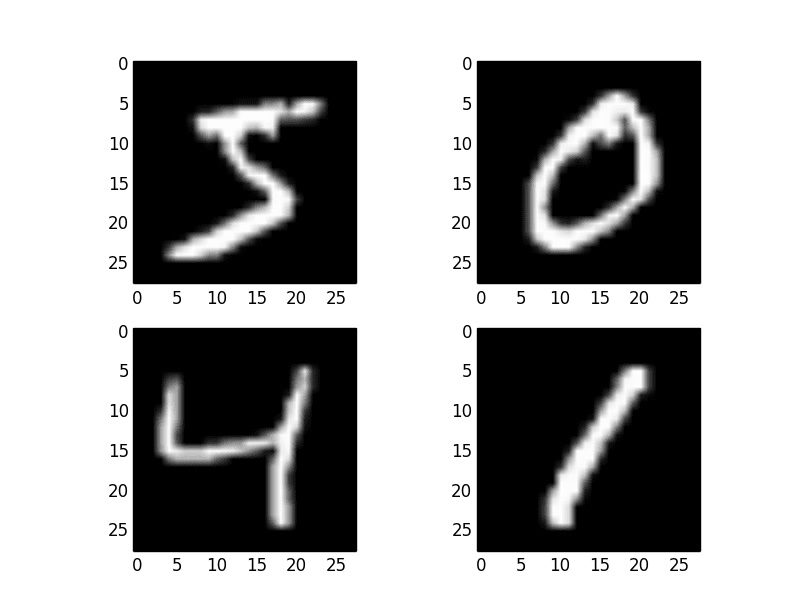
\includegraphics[width=0.7\textwidth]{mnist-handwriting-dataset.jpg}
                \caption{\label{fig:mnist-handwriting-dataset} Samples of the numbers 5, 0, 4, and 1 from the MNIST handwriting dataset.}
            \end{figure}

            Theoretically, with this data space, we can encode signifcantly more than the letters and digits in the English alphabet. An all black or all white image exists in this data space but does not represent any of the glyphs that we care about.

            The aim of data compression is to find a way of reducing the size of our data representation while preserving the ability to reconstruct the information in the original uncompressed data space at will.

            In the case of the alphabet and humans, it is quite straight forward. A person can read a character, store it in the computer as a numerical value (0-9 for `0'-`9' and 10-35 for `a'-`z'), and then when we want an image again, a human can write the digit out. But this techinque is very restricted. It can only be applied to the digit the characters the human is able to remember and that we had previously encoded as a numeric value. If the person sees a new digit they do not recognize, there is no way of storing this information using this compression format.

            We need to establish a system that is able to solve this problem, that can be performed by computers without human intervention, and that can encode more than a predefined set of discrete values (ideally a continuous spectrum of variables).

            A common techinque that has these capabilities is calles Principal Component Analysis (PCA). At a high level, it consists of finding patterns in the data (called components) and creating a system that allows us to express a datapoint in a our original data space in terms of how much of each component appears in that point.

            \ex{Compressing image of plaid patterns}{
                In this example, we will look at a set of images that consists of plaid patterns and see how PCA can be useful in reducing the amount of data it takes to store these.
            }

            

            \begin{figure}[H]
                \centering
                \begin{minipage}{0.2\textwidth}
                    \centering
                    \IApixelimage[1.25in]{
                        {3,5,5,5,5,5,5,3},
                        {5,7,7,7,7,7,7,5},
                        {5,7,7,7,7,7,7,5},
                        {5,7,7,7,7,7,7,5},
                        {5,7,7,7,7,7,7,5},
                        {5,7,7,7,7,7,7,5},
                        {5,7,7,7,7,7,7,5},
                        {3,5,5,5,5,5,5,3}%
                    }
                    Image 1
                    \label{fig:plaid_img_1}
                \end{minipage}
                \begin{minipage}{0.2\textwidth}
                    \centering
                    \IApixelimage[1.25in]{
                        {7,5,7,7,7,7,5,7},
                        {5,3,5,5,5,5,3,5},
                        {7,5,7,7,7,7,5,7},
                        {7,5,7,7,7,7,5,7},
                        {7,5,7,7,7,7,5,7},
                        {7,5,7,7,7,7,5,7},
                        {5,3,5,5,5,5,3,5},
                        {7,5,7,7,7,7,5,7}%
                    }
                    Image 2
                    \label{fig:plaid_img_2}
                \end{minipage}
                \begin{minipage}{0.2\textwidth}
                    \centering
                    \IApixelimage[1.25in]{
                        {7,7,5,7,5,7,7,7},
                        {7,7,5,7,5,7,7,7},
                        {5,5,3,5,3,5,5,5},
                        {7,7,5,7,5,7,7,7},
                        {5,5,3,5,3,5,5,5},
                        {7,7,5,7,5,7,7,7},
                        {7,7,5,7,5,7,7,7},
                        {7,7,5,7,5,7,7,7}%
                    }
                    Image 3
                    \label{fig:plaid_img_3}
                \end{minipage}
                \begin{minipage}{0.2\textwidth}
                    \centering
                    \IApixelimage[1.25in]{
                        {7,7,7,5,5,7,7,7},
                        {7,7,7,5,5,7,7,7},
                        {7,7,7,5,5,7,7,7},
                        {5,5,5,3,3,5,5,5},
                        {7,7,7,5,5,7,7,7},
                        {5,5,5,3,3,5,5,5},
                        {7,7,7,5,5,7,7,7},
                        {7,7,7,5,5,7,7,7}%
                    }
                    Image 4
                    \label{fig:plaid_img_4}
                \end{minipage}%
            \end{figure}

            The standard representation of this data would be a vector of $8 \times 8 = 64$ dimensions, where each dimension can take one of three values: 0 (black), 1 (gray) or 2 (white). This data space would have $3^64 \approx 3.43 \cdot 10^{30}$ elements but most of them would not represent plaid patterns, which is what we know our data will always represent.

            \nt{To store one of this datapoints would require storing the pixel value for each dimension, resulting in a storage size of 128 storage units.}

            What if we expressed these datapoints in a more favorable basis? Let the following be our new basis for expressing datapoints.
            
            \begin{figure}[H]
                \centering
                \begin{minipage}{0.1\textwidth}
                    \centering
                    \IApixelimage[0.65in]{
                        {5,7,7,7,7,7,7,7},
                        {5,7,7,7,7,7,7,7},
                        {5,7,7,7,7,7,7,7},
                        {5,7,7,7,7,7,7,7},
                        {5,7,7,7,7,7,7,7},
                        {5,7,7,7,7,7,7,7},
                        {5,7,7,7,7,7,7,7},
                        {5,7,7,7,7,7,7,7}%
                    }
                    Vec. 1
                \end{minipage}
                \begin{minipage}{0.1\textwidth}
                    \centering
                    \IApixelimage[0.65in]{
                        {7,5,7,7,7,7,7,7},
                        {7,5,7,7,7,7,7,7},
                        {7,5,7,7,7,7,7,7},
                        {7,5,7,7,7,7,7,7},
                        {7,5,7,7,7,7,7,7},
                        {7,5,7,7,7,7,7,7},
                        {7,5,7,7,7,7,7,7},
                        {7,5,7,7,7,7,7,7}%
                    }
                    Vec. 2
                \end{minipage}
                \begin{minipage}{0.1\textwidth}
                    \centering
                    \IApixelimage[0.65in]{
                        {7,7,5,7,7,7,7,7},
                        {7,7,5,7,7,7,7,7},
                        {7,7,5,7,7,7,7,7},
                        {7,7,5,7,7,7,7,7},
                        {7,7,5,7,7,7,7,7},
                        {7,7,5,7,7,7,7,7},
                        {7,7,5,7,7,7,7,7},
                        {7,7,5,7,7,7,7,7}%
                    }
                    Vec. 3
                \end{minipage}
                \begin{minipage}{0.1\textwidth}
                    \centering
                    \IApixelimage[0.65in]{
                        {7,7,7,5,7,7,7,7},
                        {7,7,7,5,7,7,7,7},
                        {7,7,7,5,7,7,7,7},
                        {7,7,7,5,7,7,7,7},
                        {7,7,7,5,7,7,7,7},
                        {7,7,7,5,7,7,7,7},
                        {7,7,7,5,7,7,7,7},
                        {7,7,7,5,7,7,7,7}%
                    }
                    Vec. 4
                \end{minipage}
                \begin{minipage}{0.1\textwidth}
                    \centering
                    \IApixelimage[0.65in]{
                        {7,7,7,7,5,7,7,7},
                        {7,7,7,7,5,7,7,7},
                        {7,7,7,7,5,7,7,7},
                        {7,7,7,7,5,7,7,7},
                        {7,7,7,7,5,7,7,7},
                        {7,7,7,7,5,7,7,7},
                        {7,7,7,7,5,7,7,7},
                        {7,7,7,7,5,7,7,7}%
                    }
                    Vec. 5
                \end{minipage}
                \begin{minipage}{0.1\textwidth}
                    \centering
                    \IApixelimage[0.65in]{
                        {7,7,7,7,7,5,7,7},
                        {7,7,7,7,7,5,7,7},
                        {7,7,7,7,7,5,7,7},
                        {7,7,7,7,7,5,7,7},
                        {7,7,7,7,7,5,7,7},
                        {7,7,7,7,7,5,7,7},
                        {7,7,7,7,7,5,7,7},
                        {7,7,7,7,7,5,7,7}%
                    }
                    Vec. 6
                \end{minipage}
                \begin{minipage}{0.1\textwidth}
                    \centering
                    \IApixelimage[0.65in]{
                        {7,7,7,7,7,7,5,7},
                        {7,7,7,7,7,7,5,7},
                        {7,7,7,7,7,7,5,7},
                        {7,7,7,7,7,7,5,7},
                        {7,7,7,7,7,7,5,7},
                        {7,7,7,7,7,7,5,7},
                        {7,7,7,7,7,7,5,7},
                        {7,7,7,7,7,7,5,7}%
                    }
                    Vec. 7
                \end{minipage}
                \begin{minipage}{0.1\textwidth}
                    \centering
                    \IApixelimage[0.65in]{
                        {7,7,7,7,7,7,7,5},
                        {7,7,7,7,7,7,7,5},
                        {7,7,7,7,7,7,7,5},
                        {7,7,7,7,7,7,7,5},
                        {7,7,7,7,7,7,7,5},
                        {7,7,7,7,7,7,7,5},
                        {7,7,7,7,7,7,7,5},
                        {7,7,7,7,7,7,7,5}%
                    }
                    Vec. 8
                \end{minipage}%
            \end{figure}
            \begin{figure}[H]
                \centering
                \begin{minipage}{0.1\textwidth}
                    \centering
                    \IApixelimage[0.65in]{
                        {5,5,5,5,5,5,5,5},
                        {7,7,7,7,7,7,7,7},
                        {7,7,7,7,7,7,7,7},
                        {7,7,7,7,7,7,7,7},
                        {7,7,7,7,7,7,7,7},
                        {7,7,7,7,7,7,7,7},
                        {7,7,7,7,7,7,7,7},
                        {7,7,7,7,7,7,7,7}%
                    }
                    Vec. 9
                \end{minipage}
                \begin{minipage}{0.1\textwidth}
                    \centering
                    \IApixelimage[0.65in]{
                        {7,7,7,7,7,7,7,7},
                        {5,5,5,5,5,5,5,5},
                        {7,7,7,7,7,7,7,7},
                        {7,7,7,7,7,7,7,7},
                        {7,7,7,7,7,7,7,7},
                        {7,7,7,7,7,7,7,7},
                        {7,7,7,7,7,7,7,7},
                        {7,7,7,7,7,7,7,7}%
                    }
                    Vec. 10
                \end{minipage}
                \begin{minipage}{0.1\textwidth}
                    \centering
                    \IApixelimage[0.65in]{
                        {7,7,7,7,7,7,7,7},
                        {7,7,7,7,7,7,7,7},
                        {5,5,5,5,5,5,5,5},
                        {7,7,7,7,7,7,7,7},
                        {7,7,7,7,7,7,7,7},
                        {7,7,7,7,7,7,7,7},
                        {7,7,7,7,7,7,7,7},
                        {7,7,7,7,7,7,7,7}%
                    }
                    Vec. 11
                \end{minipage}
                \begin{minipage}{0.1\textwidth}
                    \centering
                    \IApixelimage[0.65in]{
                        {7,7,7,7,7,7,7,7},
                        {7,7,7,7,7,7,7,7},
                        {7,7,7,7,7,7,7,7},
                        {5,5,5,5,5,5,5,5},
                        {7,7,7,7,7,7,7,7},
                        {7,7,7,7,7,7,7,7},
                        {7,7,7,7,7,7,7,7},
                        {7,7,7,7,7,7,7,7}%
                    }
                    Vec. 12
                \end{minipage}
                \begin{minipage}{0.1\textwidth}
                    \centering
                    \IApixelimage[0.65in]{
                        {7,7,7,7,7,7,7,7},
                        {7,7,7,7,7,7,7,7},
                        {7,7,7,7,7,7,7,7},
                        {7,7,7,7,7,7,7,7},
                        {5,5,5,5,5,5,5,5},
                        {7,7,7,7,7,7,7,7},
                        {7,7,7,7,7,7,7,7},
                        {7,7,7,7,7,7,7,7}%
                    }
                    Vec. 13
                \end{minipage}
                \begin{minipage}{0.1\textwidth}
                    \centering
                    \IApixelimage[0.65in]{
                        {7,7,7,7,7,7,7,7},
                        {7,7,7,7,7,7,7,7},
                        {7,7,7,7,7,7,7,7},
                        {7,7,7,7,7,7,7,7},
                        {7,7,7,7,7,7,7,7},
                        {5,5,5,5,5,5,5,5},
                        {7,7,7,7,7,7,7,7},
                        {7,7,7,7,7,7,7,7}%
                    }
                    Vec. 14
                \end{minipage}
                \begin{minipage}{0.1\textwidth}
                    \centering
                    \IApixelimage[0.65in]{
                        {7,7,7,7,7,7,7,7},
                        {7,7,7,7,7,7,7,7},
                        {7,7,7,7,7,7,7,7},
                        {7,7,7,7,7,7,7,7},
                        {7,7,7,7,7,7,7,7},
                        {7,7,7,7,7,7,7,7},
                        {5,5,5,5,5,5,5,5},
                        {7,7,7,7,7,7,7,7}%
                    }
                    Vec. 15
                \end{minipage}
                \begin{minipage}{0.1\textwidth}
                    \centering
                    \IApixelimage[0.65in]{
                        {7,7,7,7,7,7,7,7},
                        {7,7,7,7,7,7,7,7},
                        {7,7,7,7,7,7,7,7},
                        {7,7,7,7,7,7,7,7},
                        {7,7,7,7,7,7,7,7},
                        {7,7,7,7,7,7,7,7},
                        {7,7,7,7,7,7,7,7},
                        {5,5,5,5,5,5,5,5}%
                    }
                    Vec. 16
                \end{minipage}%
            \end{figure}
            
            If we express our datapoints as a linear combination of these vectors, then we can recreate any of the images presented above, and any other plaid pattern that we want. Importantly, we represent any pattern by just 16 values, the coefficients for each basis vector.

            With this basis, we can only represent $2^{16} = 65536$ datapoints, but those will be all the plaid pattern combinations that exists within the original dataspace. For example we can obtain the four images above by taking the following linear combinations of the basis vectors:

            \begin{figure}[H]
                \centering
                \begin{minipage}{0.1\textwidth}
                    \centering
                    \IApixelimage[0.65in]{
                        {5,7,7,7,7,7,7,7},
                        {5,7,7,7,7,7,7,7},
                        {5,7,7,7,7,7,7,7},
                        {5,7,7,7,7,7,7,7},
                        {5,7,7,7,7,7,7,7},
                        {5,7,7,7,7,7,7,7},
                        {5,7,7,7,7,7,7,7},
                        {5,7,7,7,7,7,7,7}%
                    }
                    Vec. 1
                \end{minipage}
                \begin{minipage}{0.035\textwidth}
                    \centering
                    \quad+\quad
                \end{minipage}
                \begin{minipage}{0.1\textwidth}
                    \centering
                    \IApixelimage[0.65in]{
                        {7,7,7,7,7,7,7,5},
                        {7,7,7,7,7,7,7,5},
                        {7,7,7,7,7,7,7,5},
                        {7,7,7,7,7,7,7,5},
                        {7,7,7,7,7,7,7,5},
                        {7,7,7,7,7,7,7,5},
                        {7,7,7,7,7,7,7,5},
                        {7,7,7,7,7,7,7,5}%
                    }
                    Vec. 8
                \end{minipage}
                \begin{minipage}{0.035\textwidth}
                    \centering
                    \quad+\quad
                \end{minipage}
                \begin{minipage}{0.1\textwidth}
                    \centering
                    \IApixelimage[0.65in]{
                        {5,5,5,5,5,5,5,5},
                        {7,7,7,7,7,7,7,7},
                        {7,7,7,7,7,7,7,7},
                        {7,7,7,7,7,7,7,7},
                        {7,7,7,7,7,7,7,7},
                        {7,7,7,7,7,7,7,7},
                        {7,7,7,7,7,7,7,7},
                        {7,7,7,7,7,7,7,7}%
                    }
                    Vec. 9
                \end{minipage}
                \begin{minipage}{0.035\textwidth}
                    \centering
                    \quad+\quad
                \end{minipage}
                \begin{minipage}{0.1\textwidth}
                    \centering
                    \IApixelimage[0.65in]{
                        {7,7,7,7,7,7,7,7},
                        {7,7,7,7,7,7,7,7},
                        {7,7,7,7,7,7,7,7},
                        {7,7,7,7,7,7,7,7},
                        {7,7,7,7,7,7,7,7},
                        {7,7,7,7,7,7,7,7},
                        {7,7,7,7,7,7,7,7},
                        {5,5,5,5,5,5,5,5}%
                    }
                    Vec. 16
                \end{minipage}
                \begin{minipage}{0.035\textwidth}
                    \centering
                    \quad=\quad
                \end{minipage}
                \begin{minipage}{0.1\textwidth}
                    \centering
                    \IApixelimage[0.65in]{
                        {3,5,5,5,5,5,5,3},
                        {5,7,7,7,7,7,7,5},
                        {5,7,7,7,7,7,7,5},
                        {5,7,7,7,7,7,7,5},
                        {5,7,7,7,7,7,7,5},
                        {5,7,7,7,7,7,7,5},
                        {5,7,7,7,7,7,7,5},
                        {3,5,5,5,5,5,5,3}%
                    }
                    Image 1
                \end{minipage}%
            \end{figure}

            \begin{figure}[H]
                \centering
                \begin{minipage}{0.1\textwidth}
                    \centering
                    \IApixelimage[0.65in]{
                        {7,5,7,7,7,7,7,7},
                        {7,5,7,7,7,7,7,7},
                        {7,5,7,7,7,7,7,7},
                        {7,5,7,7,7,7,7,7},
                        {7,5,7,7,7,7,7,7},
                        {7,5,7,7,7,7,7,7},
                        {7,5,7,7,7,7,7,7},
                        {7,5,7,7,7,7,7,7}%
                    }
                    Vec. 2
                \end{minipage}
                \begin{minipage}{0.035\textwidth}
                    \centering
                    \quad+\quad
                \end{minipage}
                \begin{minipage}{0.1\textwidth}
                    \centering
                    \IApixelimage[0.65in]{
                        {7,7,7,7,7,7,5,7},
                        {7,7,7,7,7,7,5,7},
                        {7,7,7,7,7,7,5,7},
                        {7,7,7,7,7,7,5,7},
                        {7,7,7,7,7,7,5,7},
                        {7,7,7,7,7,7,5,7},
                        {7,7,7,7,7,7,5,7},
                        {7,7,7,7,7,7,5,7}%
                    }
                    Vec. 7
                \end{minipage}
                \begin{minipage}{0.035\textwidth}
                    \centering
                    \quad+\quad
                \end{minipage}
                \begin{minipage}{0.1\textwidth}
                    \centering
                    \IApixelimage[0.65in]{
                        {7,7,7,7,7,7,7,7},
                        {5,5,5,5,5,5,5,5},
                        {7,7,7,7,7,7,7,7},
                        {7,7,7,7,7,7,7,7},
                        {7,7,7,7,7,7,7,7},
                        {7,7,7,7,7,7,7,7},
                        {7,7,7,7,7,7,7,7},
                        {7,7,7,7,7,7,7,7}%
                    }
                    Vec. 10
                \end{minipage}
                \begin{minipage}{0.035\textwidth}
                    \centering
                    \quad+\quad
                \end{minipage}
                \begin{minipage}{0.1\textwidth}
                    \centering
                    \IApixelimage[0.65in]{
                        {7,7,7,7,7,7,7,7},
                        {7,7,7,7,7,7,7,7},
                        {7,7,7,7,7,7,7,7},
                        {7,7,7,7,7,7,7,7},
                        {7,7,7,7,7,7,7,7},
                        {7,7,7,7,7,7,7,7},
                        {5,5,5,5,5,5,5,5},
                        {7,7,7,7,7,7,7,7}%
                    }
                    Vec. 15
                \end{minipage}
                \begin{minipage}{0.035\textwidth}
                    \centering
                    \quad=\quad
                \end{minipage}
                \begin{minipage}{0.1\textwidth}
                    \centering
                    \IApixelimage[0.65in]{
                        {7,5,7,7,7,7,5,7},
                        {5,3,5,5,5,5,3,5},
                        {7,5,7,7,7,7,5,7},
                        {7,5,7,7,7,7,5,7},
                        {7,5,7,7,7,7,5,7},
                        {7,5,7,7,7,7,5,7},
                        {5,3,5,5,5,5,3,5},
                        {7,5,7,7,7,7,5,7}%
                    }
                    Image 2
                \end{minipage}%
            \end{figure}

            \begin{figure}[H]
                \centering
                \begin{minipage}{0.1\textwidth}
                    \centering
                    \IApixelimage[0.65in]{
                        {7,7,5,7,7,7,7,7},
                        {7,7,5,7,7,7,7,7},
                        {7,7,5,7,7,7,7,7},
                        {7,7,5,7,7,7,7,7},
                        {7,7,5,7,7,7,7,7},
                        {7,7,5,7,7,7,7,7},
                        {7,7,5,7,7,7,7,7},
                        {7,7,5,7,7,7,7,7}%
                    }
                    Vec. 3
                \end{minipage}
                \begin{minipage}{0.035\textwidth}
                    \centering
                    \quad+\quad
                \end{minipage}
                \begin{minipage}{0.1\textwidth}
                    \centering
                    \IApixelimage[0.65in]{
                        {7,7,7,7,5,7,7,7},
                        {7,7,7,7,5,7,7,7},
                        {7,7,7,7,5,7,7,7},
                        {7,7,7,7,5,7,7,7},
                        {7,7,7,7,5,7,7,7},
                        {7,7,7,7,5,7,7,7},
                        {7,7,7,7,5,7,7,7},
                        {7,7,7,7,5,7,7,7}%
                    }
                    Vec. 5
                \end{minipage}
                \begin{minipage}{0.035\textwidth}
                    \centering
                    \quad+\quad
                \end{minipage}
                \begin{minipage}{0.1\textwidth}
                    \centering
                    \IApixelimage[0.65in]{
                        {7,7,7,7,7,7,7,7},
                        {7,7,7,7,7,7,7,7},
                        {5,5,5,5,5,5,5,5},
                        {7,7,7,7,7,7,7,7},
                        {7,7,7,7,7,7,7,7},
                        {7,7,7,7,7,7,7,7},
                        {7,7,7,7,7,7,7,7},
                        {7,7,7,7,7,7,7,7}%
                    }
                    Vec. 11
                \end{minipage}
                \begin{minipage}{0.035\textwidth}
                    \centering
                    \quad+\quad
                \end{minipage}
                \begin{minipage}{0.1\textwidth}
                    \centering
                    \IApixelimage[0.65in]{
                        {7,7,7,7,7,7,7,7},
                        {7,7,7,7,7,7,7,7},
                        {7,7,7,7,7,7,7,7},
                        {7,7,7,7,7,7,7,7},
                        {5,5,5,5,5,5,5,5},
                        {7,7,7,7,7,7,7,7},
                        {7,7,7,7,7,7,7,7},
                        {7,7,7,7,7,7,7,7}%
                    }
                    Vec. 13
                \end{minipage}
                \begin{minipage}{0.035\textwidth}
                    \centering
                    \quad=\quad
                \end{minipage}
                \begin{minipage}{0.1\textwidth}
                    \centering
                    \IApixelimage[0.65in]{
                        {7,7,5,7,5,7,7,7},
                        {7,7,5,7,5,7,7,7},
                        {5,5,3,5,3,5,5,5},
                        {7,7,5,7,5,7,7,7},
                        {5,5,3,5,3,5,5,5},
                        {7,7,5,7,5,7,7,7},
                        {7,7,5,7,5,7,7,7},
                        {7,7,5,7,5,7,7,7}%
                    }
                    Image 3
                \end{minipage}%
            \end{figure}

            \begin{figure}[H]
                \centering
                \begin{minipage}{0.1\textwidth}
                    \centering
                    \IApixelimage[0.65in]{
                        {7,7,7,5,7,7,7,7},
                        {7,7,7,5,7,7,7,7},
                        {7,7,7,5,7,7,7,7},
                        {7,7,7,5,7,7,7,7},
                        {7,7,7,5,7,7,7,7},
                        {7,7,7,5,7,7,7,7},
                        {7,7,7,5,7,7,7,7},
                        {7,7,7,5,7,7,7,7}%
                    }
                    Vec. 4
                \end{minipage}
                \begin{minipage}{0.035\textwidth}
                    \centering
                    \quad+\quad
                \end{minipage}
                \begin{minipage}{0.1\textwidth}
                    \centering
                    \IApixelimage[0.65in]{
                        {7,7,7,7,5,7,7,7},
                        {7,7,7,7,5,7,7,7},
                        {7,7,7,7,5,7,7,7},
                        {7,7,7,7,5,7,7,7},
                        {7,7,7,7,5,7,7,7},
                        {7,7,7,7,5,7,7,7},
                        {7,7,7,7,5,7,7,7},
                        {7,7,7,7,5,7,7,7}%
                    }
                    Vec. 5
                \end{minipage}
                \begin{minipage}{0.035\textwidth}
                    \centering
                    \quad+\quad
                \end{minipage}
                \begin{minipage}{0.1\textwidth}
                    \centering
                    \IApixelimage[0.65in]{
                        {7,7,7,7,7,7,7,7},
                        {7,7,7,7,7,7,7,7},
                        {7,7,7,7,7,7,7,7},
                        {5,5,5,5,5,5,5,5},
                        {7,7,7,7,7,7,7,7},
                        {7,7,7,7,7,7,7,7},
                        {7,7,7,7,7,7,7,7},
                        {7,7,7,7,7,7,7,7}%
                    }
                    Vec. 12
                \end{minipage}
                \begin{minipage}{0.035\textwidth}
                    \centering
                    \quad+\quad
                \end{minipage}
                \begin{minipage}{0.1\textwidth}
                    \centering
                    \IApixelimage[0.65in]{
                        {7,7,7,7,7,7,7,7},
                        {7,7,7,7,7,7,7,7},
                        {7,7,7,7,7,7,7,7},
                        {7,7,7,7,7,7,7,7},
                        {7,7,7,7,7,7,7,7},
                        {5,5,5,5,5,5,5,5},
                        {7,7,7,7,7,7,7,7},
                        {7,7,7,7,7,7,7,7}%
                    }
                    Vec. 14
                \end{minipage}
                \begin{minipage}{0.035\textwidth}
                    \centering
                    \quad=\quad
                \end{minipage}
                \begin{minipage}{0.1\textwidth}
                    \centering
                    \IApixelimage[0.65in]{
                        {7,7,7,5,5,7,7,7},
                        {7,7,7,5,5,7,7,7},
                        {7,7,7,5,5,7,7,7},
                        {5,5,5,3,3,5,5,5},
                        {7,7,7,5,5,7,7,7},
                        {5,5,5,3,3,5,5,5},
                        {7,7,7,5,5,7,7,7},
                        {7,7,7,5,5,7,7,7}%
                    }
                    Image 4
                \end{minipage}%
            \end{figure}

        \section{A linear algebra analogy}
            We can draw the analogy from the abstract high-level concepts that we just looked at the change of basis procedures that we studied in class. As mentioned, above, each datapoint is a vector, and an ``expression system'' is simply a set of basis vectors that can be used to write out datapoints in an expressed form.

            By the theorem seen in class, if one has the same number of linearly independent vectors as dimensions in a space, that set of vectors forms a basis. But it we find a set of $n$ vectors, to represent datapoints in an $n$ dimensional space, we have achieved no compression, since we can use the standard basis and obtain the same storage efficiency.
            
            Ideally the dataset that we want to represent only contains vectors in a lower-dimensional subspace of the data space. That way, we can express all the data points we are interested with a smaller number of vectors.
            
            Unfortunately, real world data rarely fits a proper mathematical subspace, so this technique would not be reliable for all types of data. For example, assume all our data is on a plane within a 3-dimensional data space. With just one point that is not within the plane, we have increased the dimension of our subspace to 3, yielding not compression when expressing datapoints with new eigenvectors.
            
            Our method must take into account how ``important'' these areas of space are to decide whether it is worth reducing our compression efficiency to be able to represent only a few infrequent datapoints.
                
            \Inote{Use our variance knowledge from example image to say that some sections of the image have less information (the constant ones) and some have more information (the ones that vary widely)}
        
        \section{Formalizing the calculation of ``high information'' eigenvectors}
            \Lnote{change wording so that this applies to handwriting recognition instead of face recognition}
            The motivation for using principal component analysis is to find what Turk and Pentland referred to as ``face space\Knote{I think more explanation of face space might help understanding},'' and which in our case we can conceptualize as the data space of letters. The face images, as previously explained, live as vectors in large dimensional spaces ($65,536$-dimensional \Knote{We certainly do not want to work with that!} space for a typical image). The goal at this stage is to reduce our large input vector space to a lower dimensional subspace that can be described be an eigenbasis.  
    
            \Knote{is this also kinda defined in chapter 2?}

            \dfn{Covariance}{
                In order to construct... we need to define the \textbf{covariance}.  Covariance measures the overall correlation between certain variables. The covariance $\sigma$ of two variables, $X$ and $Y$, is defined
                    \[\sigma(X,Y) = \frac{1}{M} \sum _{i=1}^{M} (X_i-\IAmean{X}) (Y_i-\IAmean{Y})\]
            }
    
            \dfn{Covariance Matrix}{
                \textbf{Covariance matrix}, then, is a matrix that measures the covariance of various variables.
                
                For variables $x_1,\ldots,x_p$, the covariance matrix is defined as follows
                \[
                    C = \IAmatrix{
                        \sigma_{11} & \sigma_{12} & ... & \sigma_{1p} \\
                        \sigma_{21} & \sigma_{22} &  & \\
                        \vdots  &  & \ddots  & \\
                        \sigma_{p1} &  &  & \sigma _{pp}
                    }
                \]
                
                where $\sigma_{ij}$ represents the covariance between the $i^{th}$ and $j^{th}$ variable. In the case of eigenfaces, the $p$ independent variables correspond to our $N^{2}$ bits, and thus $p$ corresponds to the dimension of our images. 
            }
            
            Having thus defined our covariance matrix, we must now discuss why we are taking the eigenvectors of this particular matrix to be our eigenfaces. In order for our eigenfaces to be as efficient as possible, we want each eigenface to encode as much variance as possible. 
            
            We take eigenvectors to simplify a relation defined by matrix multiplication to a relation defined by scalar multiplication, so that we may write any face as a linear combination of eigenvectors. Taking an eigenvector $e$, $C e = \lambda e$. If $\lambda$ is large, then the covariance between $e$ and all many other faces is high. If $\lambda$ is small, then the covariance is less. Therefore, we will see later that we want to prioritize large eigenvalues when constructing our eigenbasis. 
            
            Before we discuss the eigenvalues, however, we must derive some more definitions of $C$.
            
            Firstly, given the large size of $N^2$ \Knote{Is this N previously defined} , it is convenient for us to find a more condensed description of the covariance matrix
    
            \thm{}{
                Let $C$ be a $p \times p$ covariance matrix where each element $c_{ij} = \sigma_{ij}$. Let $\Phi_a = P_a - \IAmean{P}$, where
                    \[
                        P_a = \IAmatrix{
                            x_{1a} \\
                            x_{2a} \\
                            \vdots \\
                            x_{pa}
                        }
                    \]
                with $a$ from $1$ to $M$.
                
                Then $C = \frac{1}{M} \sum_{a=1}^M \Phi_a \Phi_a^T$.
            }
            \begin{myproof}
                We can prove this theorem starting with
                    \[
                        C = \IAmatrix{
                            \sigma_{11} & \sigma_{12} & \cdots & \sigma_{1p} \\
                            \sigma_{21} & \sigma_{22} &        &             \\
                            \vdots      &             & \ddots &             \\
                            \sigma_{p1} &             &        & \sigma_{pp}
                        }
                    \]
        
                From the definition of covariance, each entry $c_{ij} = \frac{1}{M} \sum _{i=1}^M \left( x_{ia} - \IAmean{x_i}\right) \left(x_{ia} - \IAmean{x_i}\right)$. Since matrices add linearly, we can factor out the summation $\frac{1}{M} \sum_{i=1}^M$. Thus we can write
                    \[
                        C = \frac{1}{M} \sum_{i=1}^M \IAmatrix{
                            \left(x_{1a} - \IAmean{x}_1\right) \left(x_{1a} - \IAmean{x}_1\right) & \dotsc  & \left(x_{1a} - \IAmean{x}_1\right) \left(x_{pa} - \IAmean{x}_p\right) \\
                            \vdots & \ddots & \\
                            \left(x_{pa} - \IAmean{x}_p\right) \left(x_{1a} - \IAmean{x}_1\right) &  & \left(x_{pa} - \IAmean{x}_p\right) \left(x_{pa} - \IAmean{x}_p\right)
                        }
                    \] \Inote{Clarify notation because $\IAmean{x}_p$ is not defined anywhere}
                
                
                Now consider the term $\Phi_a \Phi_a^T = (P_i - \IAmean{P}) (P_i - \IAmean{P})^T$, as defined in the theorem. Since the transpose operator is distributive,
                    \[
                        (P_i - \IAmean{P}) (P_i - \IAmean{P})^T =
                            \left(
                                \IAmatrix{
                                    x_{1a} \\
                                    x_{2a} \\
                                    \vdots \\
                                    x_{pa}
                                } - \IAmean{P}
                            \right) \left(
                                \IAmatrix{
                                    x_{1i} & x_{2i} & \dotsc & x_{pi}
                                } - \IAmean{P}^T
                            \right)
                    \]
                    \[
                        =
                            \left(
                                \IAmatrix{
                                    x_{1a} \\
                                    x_{2a} \\
                                    \vdots \\
                                    x_{pa}
                                } - \IAmatrix{
                                    \IAmean{x}_1 \\
                                    \IAmean{x}_2\\
                                    \vdots \\
                                    \IAmean{x}_p
                                }
                            \right) \left(
                                \IAmatrix{
                                    x_{1a} & x_{2a} & \dotsc & x_{pa}
                                } - \IAmatrix{
                                    \IAmean{x}_1 & \IAmean{x}_2 & \dotsc & \IAmean{x}_p
                                }
                            \right)
                    \]
                    \[
                        =
                            \IAmatrix{
                                x_{1a} - \IAmean{x}_1 \\
                                x_{2a} - x_2 \\
                                \vdots \\
                                x_{pa} - \IAmean{x}_p
                            }
                            \IAmatrix{
                                x_{1a} - \IAmean{x}_1 & x_{2a} - \IAmean{x}_2 & \dotsc & x_{pa} -\IAmean{x}_p
                            }
                    \]
                
                Therefore,
                    \[
                        \Phi_a {\Phi_a}^T = \IAmatrix{
                            \left(x_{1a} - \IAmean{x}_1\right)\left(x_{1a} - \IAmean{x}_1\right) & \dotsc & \left(x_{1a} - \IAmean{x}_1\right) \left(x_{pa} - \IAmean{x}_p\right) \\
                            \vdots & \ddots & \\
                            \left(x_{pa} - \IAmean{x}_p\right) \left(x_{1a} - \IAmean{x}_1\right) & & \left(x_{pa} - \IAmean{x}_p\right) \left(x_{pa} - \IAmean{x}_p\right)
                        }
                    \]
                    \[
                        C = \frac{1}{M} \sum_{a=1}^M \Phi_a {\Phi_a}^T
                    \]
            \end{myproof}
            
            By constructing 
            
            \href{https://builtin.com/data-science/step-step-explanation-principal-component-analysis}{REFERENCE PRINCIPAL COMPONENT ANALYSIS}
            
            In the eigenface case, we wish to measure the difference between our face vectors $\Gamma_i$ differ from the average face. We can define the average face $\IAmean{\Gamma}$ as follows,
                \[
                    \IAmean{\Gamma} = \frac{1}{M} \sum_{n=1}^M \Gamma_n
                \]
    
            We can write the difference $\Phi_i$ between the average face and the $i^{th}$ face,
                \[
                    \Phi_i = \Gamma_i - \IAmean{\Gamma}
                \]
            
            \href{https://nzmaths.co.nz/category/glossary/variance-discrete-random-variable\#:\textasciitilde:text=A\%20measure\%20of\%20spread\%20for,2\%20or\%20\%CF\%832x.}{Hello}
            
            \thm{}{
                Let $C$ be an $N^2 \times N^2$ covariance matrix, defined as $C = \frac{1}{M} \sum_{n=1}^M \Phi_n \Phi_n^T$, where $M$ is the dimension of the domain $C$. Let $A$ be an $N^2 \times N^2$ matrix with columns $[\Phi_1 \ \Phi_2 \ \dots \Phi_M]$.
                
                Then $C = A A^T$.
            }
    
            \begin{myproof}
                
            \end{myproof}
            
            Going back to our matrix $C$,
                \[
                    C = \IAmatrix{
                        \sigma_{11} & \sigma_{12} & \dots  & \sigma_{1p} \\
                        \sigma_{21} & \sigma_{22} &        &             \\
                        \vdots      &             & \ddots &             \\
                        \sigma_{p1} &             &        & \sigma_{pp}
                    }
                \]
    
             We can expand $C$ according to the definition of $\sigma$,
                \[
                    C = \frac{1}{M} \sum_{a=1}^M \IAmatrix{
                        \Phi_1 {\Phi_1}^T & \Phi_1 \Phi_2^T   & \dots  & \Phi_1 {\Phi_p}^T \\
                        \Phi_2 {\Phi_1}^T & \Phi_2 {\Phi_2}^T &        &                   \\
                        \vdots            &                   & \ddots &                   \\
                        \Phi_p {\Phi_1}^T &                   &        & \Phi_p {\Phi_p}^T
                    }
                \]
        
            \Anote{...}
            
            Now we can express our eigenvectors $v_{i}$ and eigenvalues $\lambda _{i}$ as
                \[
                    \lambda_i v_i = A A^T v_i
                \]
    
            However, $A A^T$ is an $N^2$by $N^2$ matrix (where $N \times N$ is the resolution of the image), which for images of any discernable resolution will be much larger than desired in order to compute its eigenvectors. 
            
            Let
                \[
                    S = A A^T = \lambda_i v_i
                \]
    
            Then,
                \[
                    S^T = \left(A A^T\right)^T = A^T A
                \]
    
            We can show that $S$ and $S^{T}$ have the same eigenvalues. 
            
            Since the indetity matrix is symmetrical, since the transpose operation is distributive, and since $\det(A) = \det\left(A^T\right)$,
                \[
                    \det\left(S^T - \lambda_i I\right) = \det(S - \lambda_i I)^T = \det(S - \lambda_i I)
                \]
            and therefore $S$ and $S^T$ have the same eigenvalues.
            
            Applying this to our eigenfaces,
                \[
                    S^T = A^T A = \lambda_i u_i
                \]
    
            The advantage of effectively reordering the $A$ and $A^T$ is that our new matrix $S^T$ is an $M \times M$ matrix. $M$ corresponds to the size of the training set, which in most cases is much smaller than the dimension of the resolution of the image. Therefore, it will be much easier to compute the eigenfaces. We can then write each face as a linear combination of the eigenfaces
            
            \href{https://datascienceplus.com/understanding-the-covariance-matrix/}{MEGAREFERENCE}
            
            \[
                \Gamma_i = \sum_{n=1}^M c_{in} u_{n}
            \]
    
            We can interpret the eigenvectors of the covariance matrix as vectors that encode the greatest variance in data, and as such are the most suited for reconstructing faces from (ghosts). The corresponding eigenvalues tell how much variance each eigenvector encodes. For this reason, the greater the eigenvalue the more adaptable and better suited the eigen vector. When choosing eigenvectors to form a basis for the eigenspace used for facial recognition, one therefore prioritizes them by eigenvalue from highest to lowest.
            
            \href{http://math.clarku.edu/\textasciitilde djoyce/ma217/covar.pdf}{AWDAWD}
            \Knote{This section was a little confusing. I understand that there are still sections missing but I think if it were tied back to the information extraction it would make more sense. Relating it back would kind of answer the question of why we are doing all this simplification and proofs. }
    
    \chapter{Uses Beyond Compression}
    We mainly discussed how PCA allows us to reduce the dimensions of our data space and store data more efficiently, but there are more uses for this beyond compression. Having a simpler representation for our data allows us to perform more complex operations on it.

    \section{Classification}
    We can use PCA to perform classification on our data. After we have chosen our eigenvectors based on our initial dataset, and have manually classified the original ``training'' data into categories, we can use Linear Classification \cite{Milon2019} to classify new data into the preexisting categories.

    This process consists of projecting the new datapoint to our lower-dimension subspace and then making a category decision based on how much weight each basis vector has in the new datapoint.

    \section{Recognition}
    In cases were there are no discrete categories defined during training time, we can use dimensionality reduction to more easily (and faster) compare a new datapoint to a list of known datapoints that continually gets updates.

    In the case of facial recognition, we can use PCA to reduce the dimensionality of our data and then use a distance metric to compare the new datapoint to the known datapoints. The datapoint with the smallest distance to the new datapoint is the most similar and is therefore the most likely to be the same person.

    % \chapter{Discussion}
    % \section{Is this software Anglo-centric?}
    % \blindtext[1]
    
    \pagebreak
    
    % ================ %
    % == References == %
    % ================ %
    \bibliographystyle{alpha}
    \bibliography{sample}
    
\end{document}